\subsection{Benchmarking Generative Models on 2D Airfoils}
\label{ch6:sec:benchmarking}

Generative adversarial networks (GANs) and variational autoencoders (VAEs) represent two state-of-the-art frameworks for data-driven aerodynamic design space exploration. To benchmark \textit{DiffGeo}’s diffusion-based approach, we compare it against these baselines on a common task of 2D airfoil generation. Importantly, all models operate within the same learned shape parameterization: the automatic latent space model (LSM) introduced by ~\citet{aa.Wei2023,aa.Wei2023b}. The advantages of this automatic LSM have been thoroughly discussed in prior work. Using a shared latent representation ensures a fair comparison by isolating the effect of the sampling mechanism from differences in geometry encoding. We examine three key aspects of generative performance:

\begin{itemize}
    \item \textbf{LSDM vs. Adversarial Training}: Both \textit{DiffGeo} and the GAN baseline generate airfoils by sampling in the latent space learned by the LSM. The GAN uses adversarial training to produce latent codes, while \textit{DiffGeo} uses a latent space diffusion model (LSDM) for more stable and data-efficient sampling. We compare how these approaches perform, particularly when training data is extremely limited.

    \item \textbf{Generative Sampling vs. VAE Prior}: Unlike LSDM and GANs which rely on explicit external samplers, a VAE-style model integrates sampling by learning a Gaussian prior in the latent space. For comparison, we adapt the LSM into a variational auto-decoder (VAD) to enforce a learned latent Gaussian distribution (similar to a VAE) and evaluate whether this prior-based sampling strategy affects output diversity and quality differently than LSDM’s learned sampler.

    \item \textbf{Energy-Based Guidance vs. Conditional GAN}: \textit{DiffGeo}’s conditional extension CLSDM uses energy-based guidance during sampling to incorporate constraints without retraining the generator. In contrast, a conditional GAN (CGAN) baseline requires paired data and retraining to implement new conditions. We assess each model’s ability to satisfy design constraints under limited data--comparing CLSDM’s flexible, plug-and-play guidance to CGAN’s fixed, learned conditioning.
\end{itemize}


\subsubsection{Generative Adversarial Network Baseline}
For the GAN baseline, we implement a generator–discriminator pair that shares the LSM latent space with \textit{DiffGeo}. 

The generator $g_{\Gamma}^{(G)}: \mathbb{R}^d \to \bZ$ is a multilayer perceptron (MLP) that maps a random Gaussian noise $\epsilon \sim \cN(\mathbf{0},\bI)$ to a latent code $\bz = g^{(G)}_\Gamma(\mathbf{\epsilon})$. It uses the same architecture as \textit{DiffGeo}’s diffusion network, but is trained via an adversarial objective. The discriminator $g_{\Pi}^{(D)}: \bZ \rightarrow [0,1]$ is an MLP that attempts to distinguish `real' latent codes $\bz_{\text{real}}$ obtained by auto-decoding from training data, from `fake' codes generated by $g^{(G)}_\Gamma$. It consists of two hidden layers, which is an empirical setting for stable adversarial training. Both networks are trained with the standard \textit{minimax} objective~\cite{ai.Goodfellow2020} using the AdamW optimizer and a learning rate of $10^{-5}$:
\begin{equation}
    \min_\Gamma \max_\Pi = 
    \mathbb{E}_{\hat{\bz}_\text{real} \sim p_{data}} \left[ \log g^{(D)}_\Pi(\hat{\bz}_\text{real}) \right] + 
    \mathbb{E}_{\mathbf{\epsilon} \sim \cN(\mathbf{0}, \bI)} \left[ \log \left( 1 - g^{(D)}_\Pi( g^{(G)}_\Gamma(\mathbf{\epsilon}) ) \right)\right]\;,
\end{equation}

After training, the GAN generator can produce new latent samples $\bz=g^{(G)}(\mathbf{\epsilon})$, which are then decoded by the LSM’s decoder to obtain a new airfoil $M=\{\hat{V} + f_{\Theta}(\bz, \hat{V}), E\}$, where $\bar{V}$ are template mesh vertices and $f_{\Theta}$ is the LSM's deformation function.

We also implement a conditional GAN (CGAN) variant for comparisons. The CGAN generator and discriminator are augmented to accept a conditioning input $C$ (e.g., a target parameter) as $g_{\Gamma}^{(G)}(\mathbf{\epsilon},C)$ and $g_{\Pi}^{(D)}(\bz,C)$. This allows GAN sampling under a given condition by learning through training on paired data, though it lacks the flexibility of \textit{DiffGeo}’s energy-based conditioning.

\subsubsection{Variational Auto-Decoder Baseline}
As a second generative baseline, we convert the LSM into a variational latent model similar to a VAE, but without an encoder network. Specifically, we treat each training shape $S_1,\dots,S_K$ as having its own latent distribution rather than a fixed code, thereby creating a variational auto-decoder (VAD). During training, we optimize the decoder’s weights $\Theta$ and learn a mean $\mathbf{\mu}_i\in \mathbb{R}^d$ and standard deviation $\mathbf{\sigma}_i\in \mathbb{R}^d_{>0}$ for the latent vector of each training shape $S_i$. This effectively enforces a Gaussian prior in the latent space: the learned $\{\mathbf{\mu}_i, \mathbf{\sigma}_i\}$ approximate the shape’s posterior, and a new latent code $\bz_i$ can be sampled by perturbing these distributions using the reparameterization trick:

\[\bz_k=\mathbf{\mu}_i+\mathbf{\sigma}_i\mathbf{\epsilon}, \quad \mathbf{\epsilon\sim \cN(\mathbf{0}, \bI)}\;.\]

The sampled latent code is passed to VAD's decoder $f^{V}_\theta$ to generate deformed airfoil. The model is trained to minimize the loss:
\begin{equation*}
    \min_{\Theta,\{\mathbf{\mu}_i, \mathbf{\sigma}_i\}} \;
  \sum_{i=1}^K \left[
    \cL_{CD}(\hat{V}+f^V_{\Theta}(\bz_i), S_i) 
    + \cD_{KL}\bigl(\cN(\mathbf{\mu}_i, \operatorname{diag}(\mathbf{\sigma}_i^2)) \,\|\, \cN(\mathbf{0}, \bI)\bigr)
  \right].
\end{equation*}
The chamfer distance $\cL_{CD}$ minimizes the reconstruction error, while the Kullback–Leibler divergence $\cD_{KL}$ regularizes the latent space toward a standard normal prior. The reparameterization allows gradients to flow through stochastic sampling and enables end-to-end training.

We use the same decoder architecture as the original LSM, training $\Theta$ with a learning rate of $5\times10^{-4}$, while the latent distribution parameters ${\mathbf{\mu}_i,\mathbf{\sigma}_i}$ are updated with a higher learning rate $10^{-3}$. The VAD baseline integrates the sampling mechanism into the model via the learned Gaussian priors, providing a point of comparison for \textit{DiffGeo}’s external sampler LSDM versus an internal latent prior approach.

\subsubsection{Data Preparation}
We collect airfoils from the UIUC database~\cite{aa.Selig1996}, which offers a wide variety of foil profiles. Six subsets are randomly sampled, each consisting of $1000$, $500$, $250$, $100$, and $50$ airfoils, respectively.
%For simplicity, we use the notion `<\textit{model name}>-<\textit{training data number}>' to represent the model's type and the training setting, such as `LSDM-1k' and `GAN-100'.
%For conditional models, we append another item `<\textit{condition}>', such as `CLSDM-500-MT12' for airfoil's maximum thickness constrained to $12\%$ chord length or 'CGAN-100-A0.05' for airfoil's area constrained to $0.05$.


\begin{figure}[!t]
    \begin{center}
        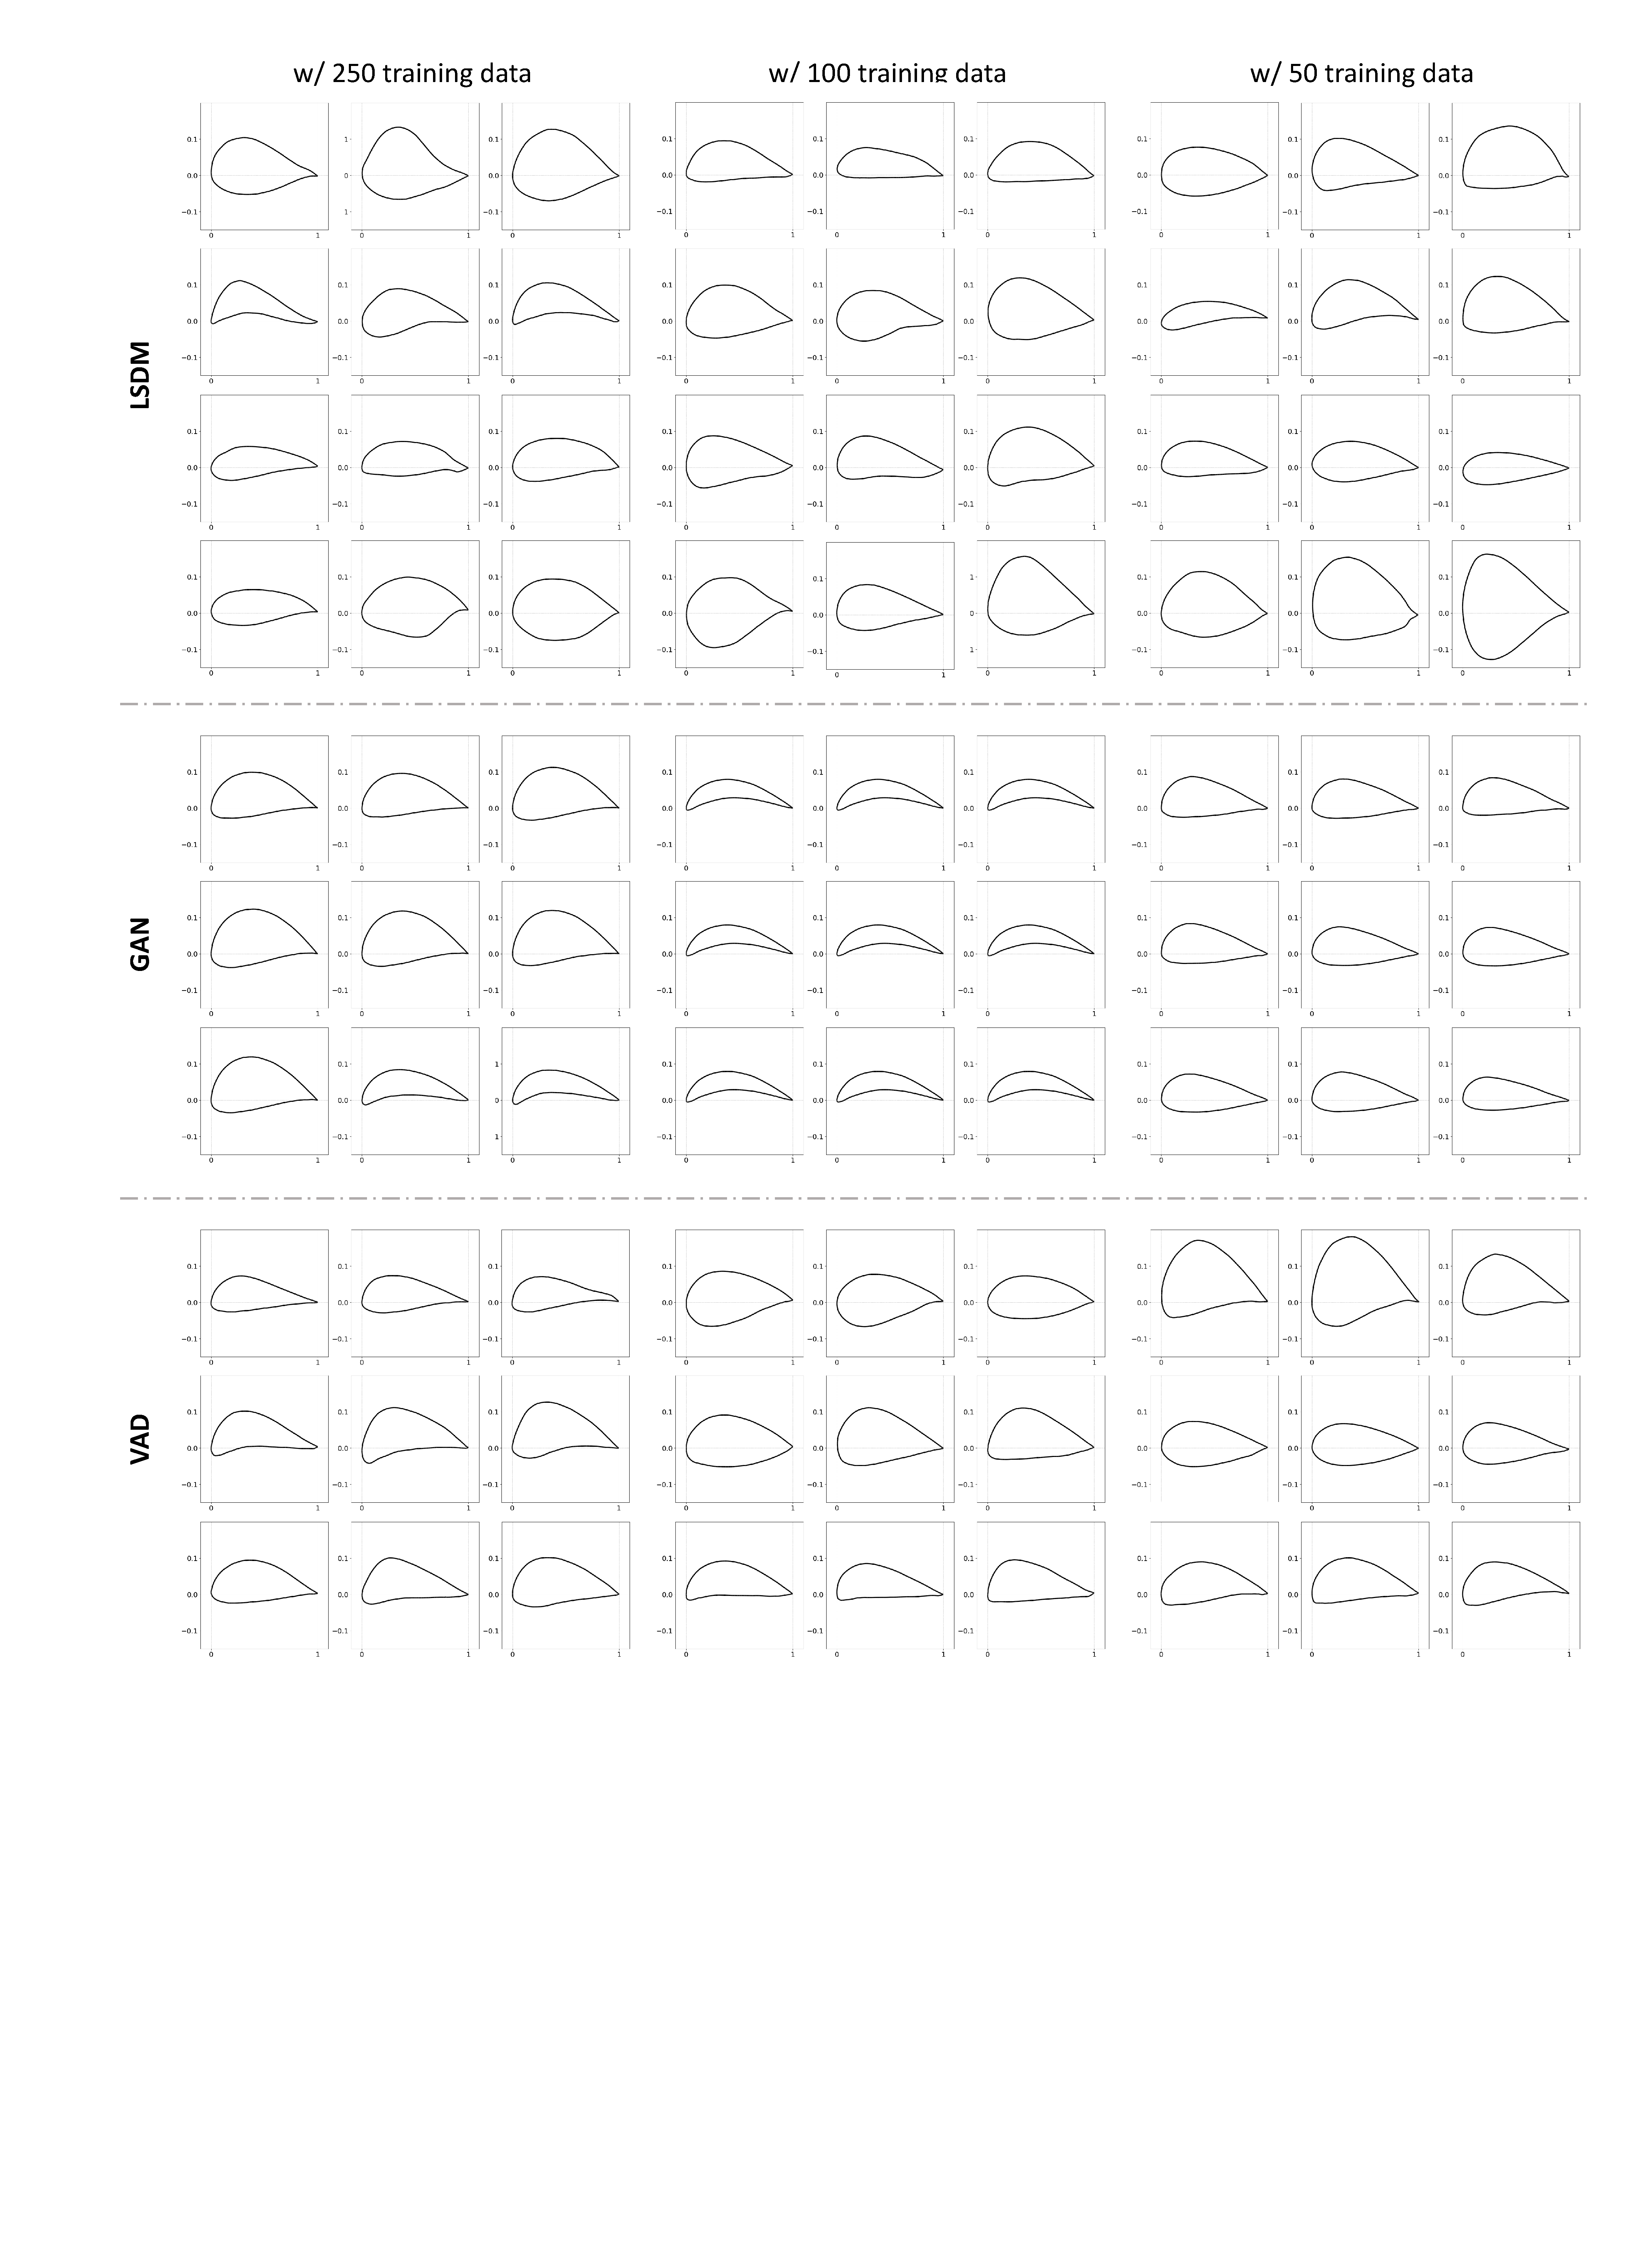
\includegraphics[width=1\linewidth]{chapter6/fig/fig_uncon_airfoils_updated.pdf}
    \end{center}
    \caption{
        \small Unconditional airfoil samples generated by GAN, VAD and LSDM.
    }
    \label{ch6:fig:main_unconditional_airfoils}
\end{figure}

\begin{figure}[!t]
    \begin{center}
        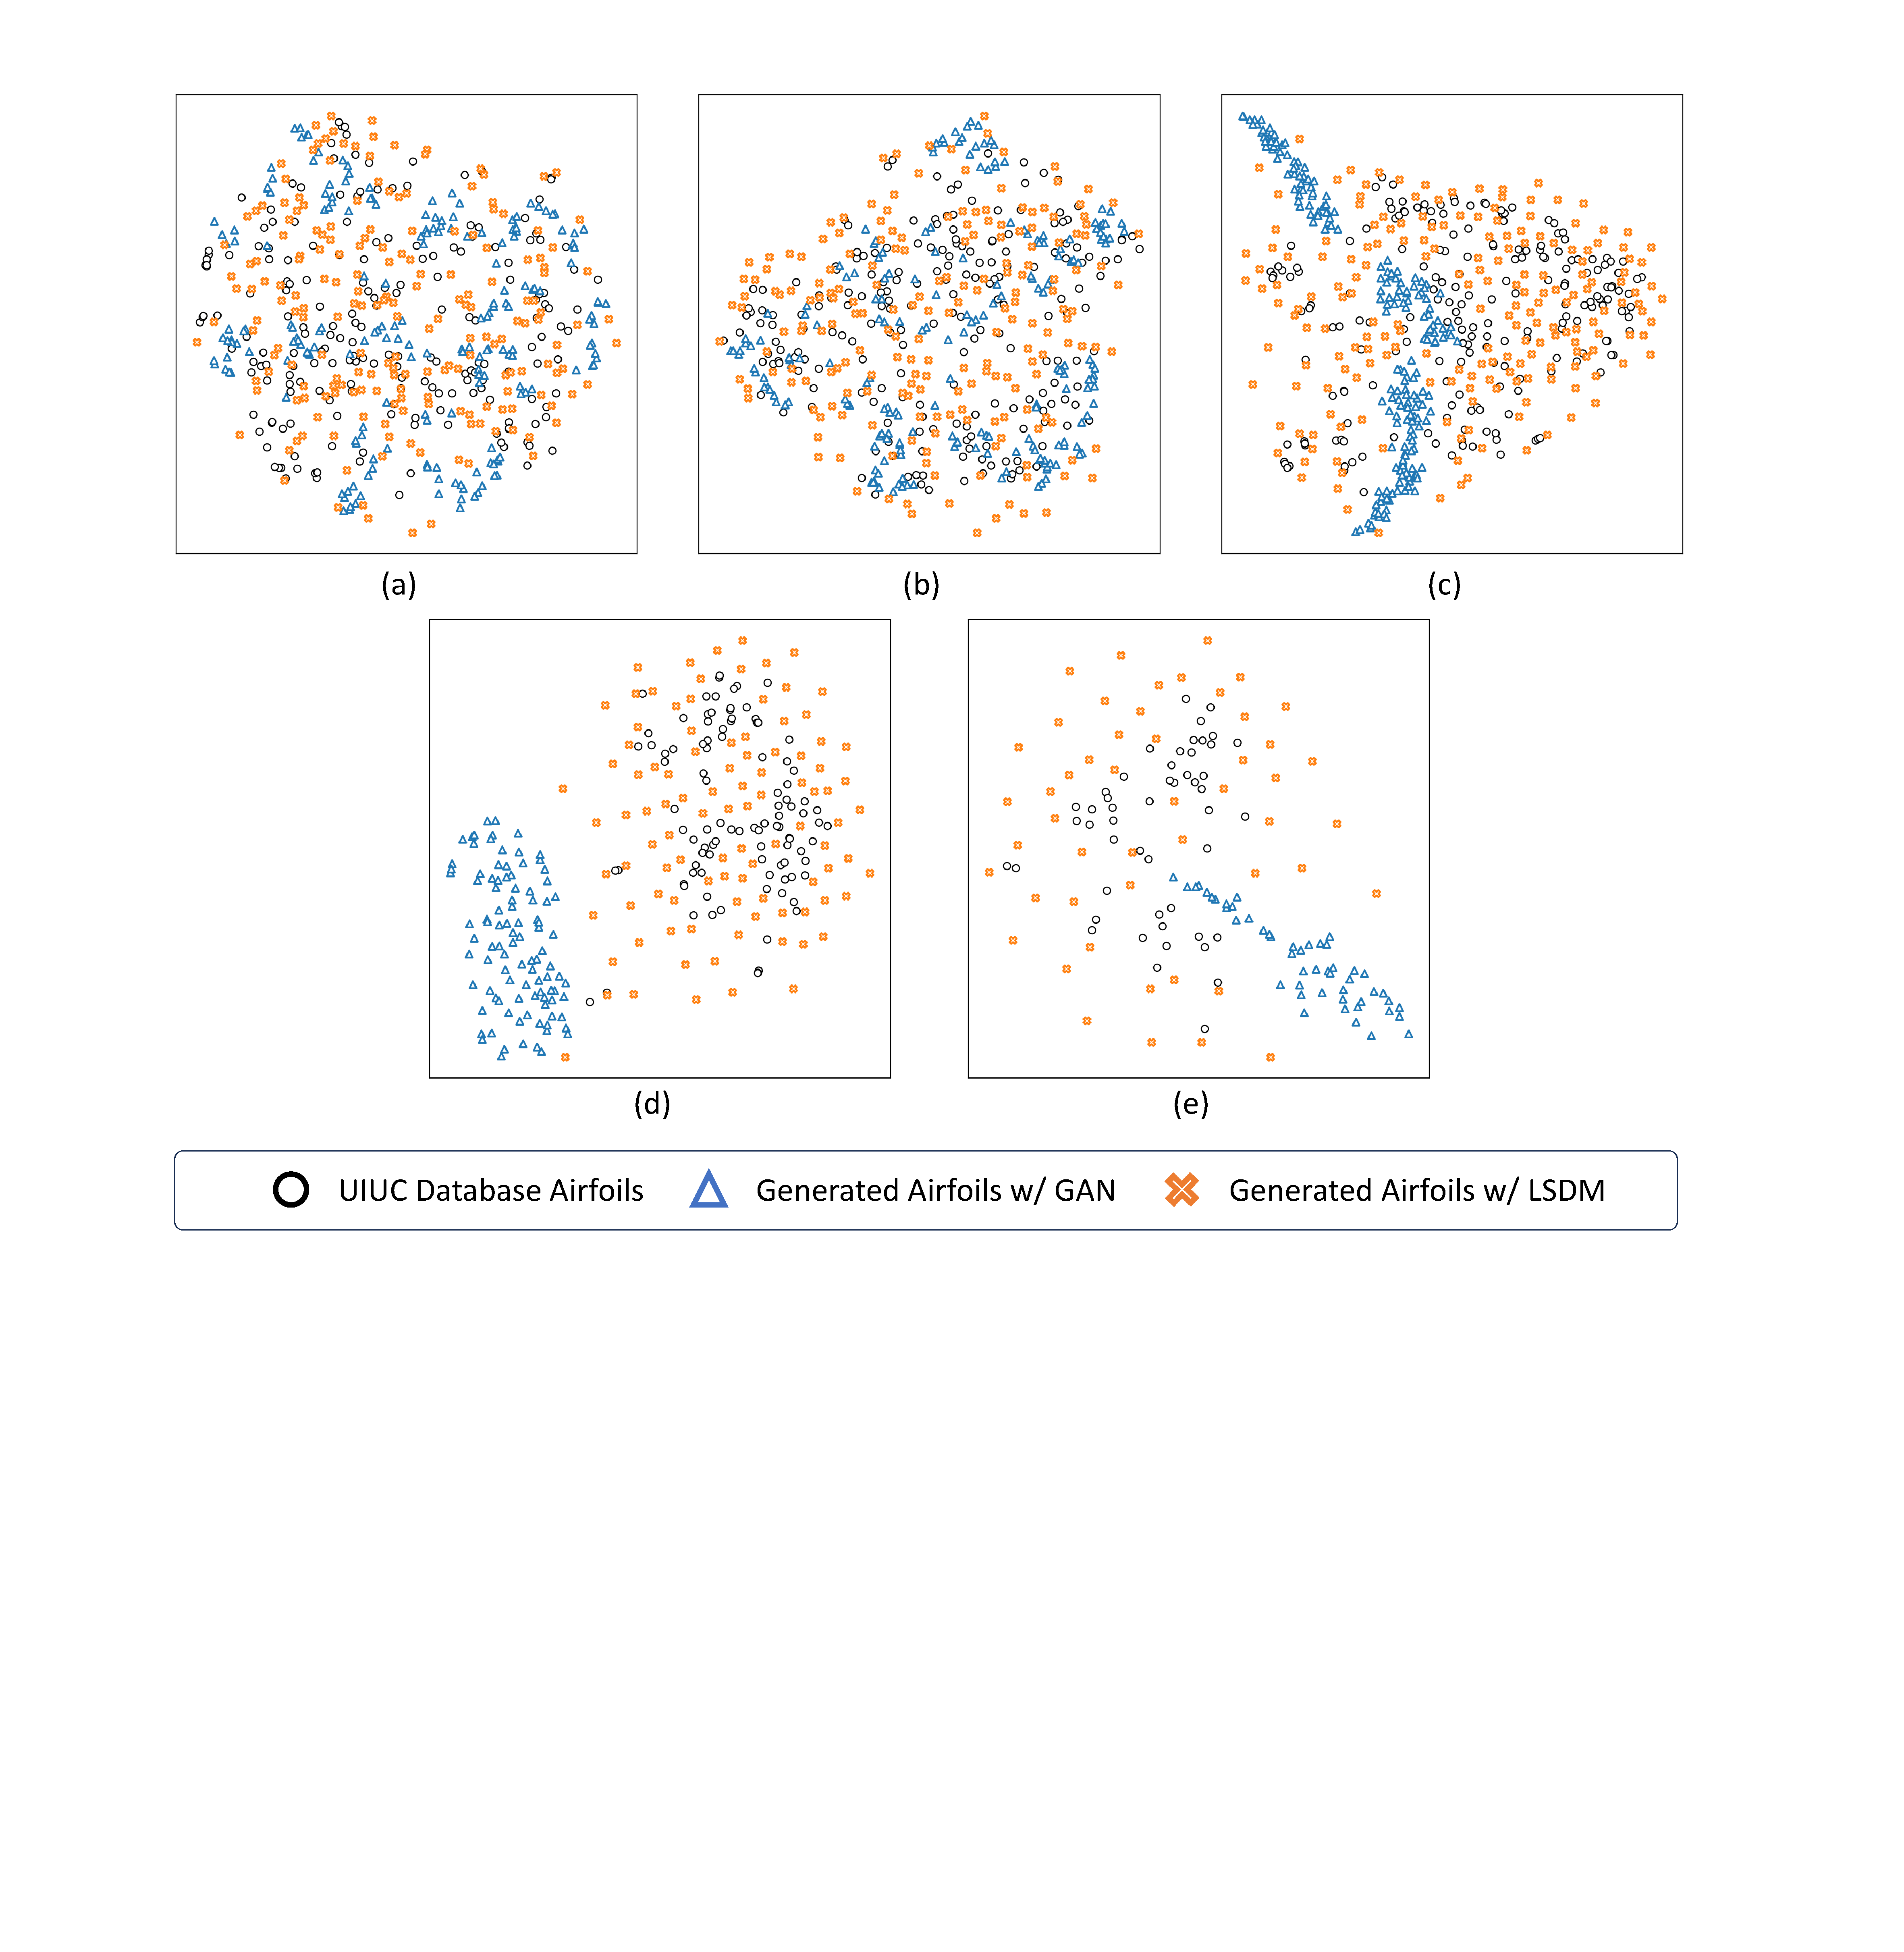
\includegraphics[width=0.95\linewidth]{chapter6/fig/unconditional_tsne.pdf}
    \end{center}
    \caption{
        \small \textit{t-SNE} visualization of airfoils' latent codes from UIUC database, LSDM and GAN for training sizes of (a) $1000$, (b) $500$, (c) $250$, (d) $100$ and (e) $50$ airfoils.
    }
    \label{ch6:fig:main_unconditional_tsne}
\end{figure}

\begin{figure}[!h]
    \begin{center}
        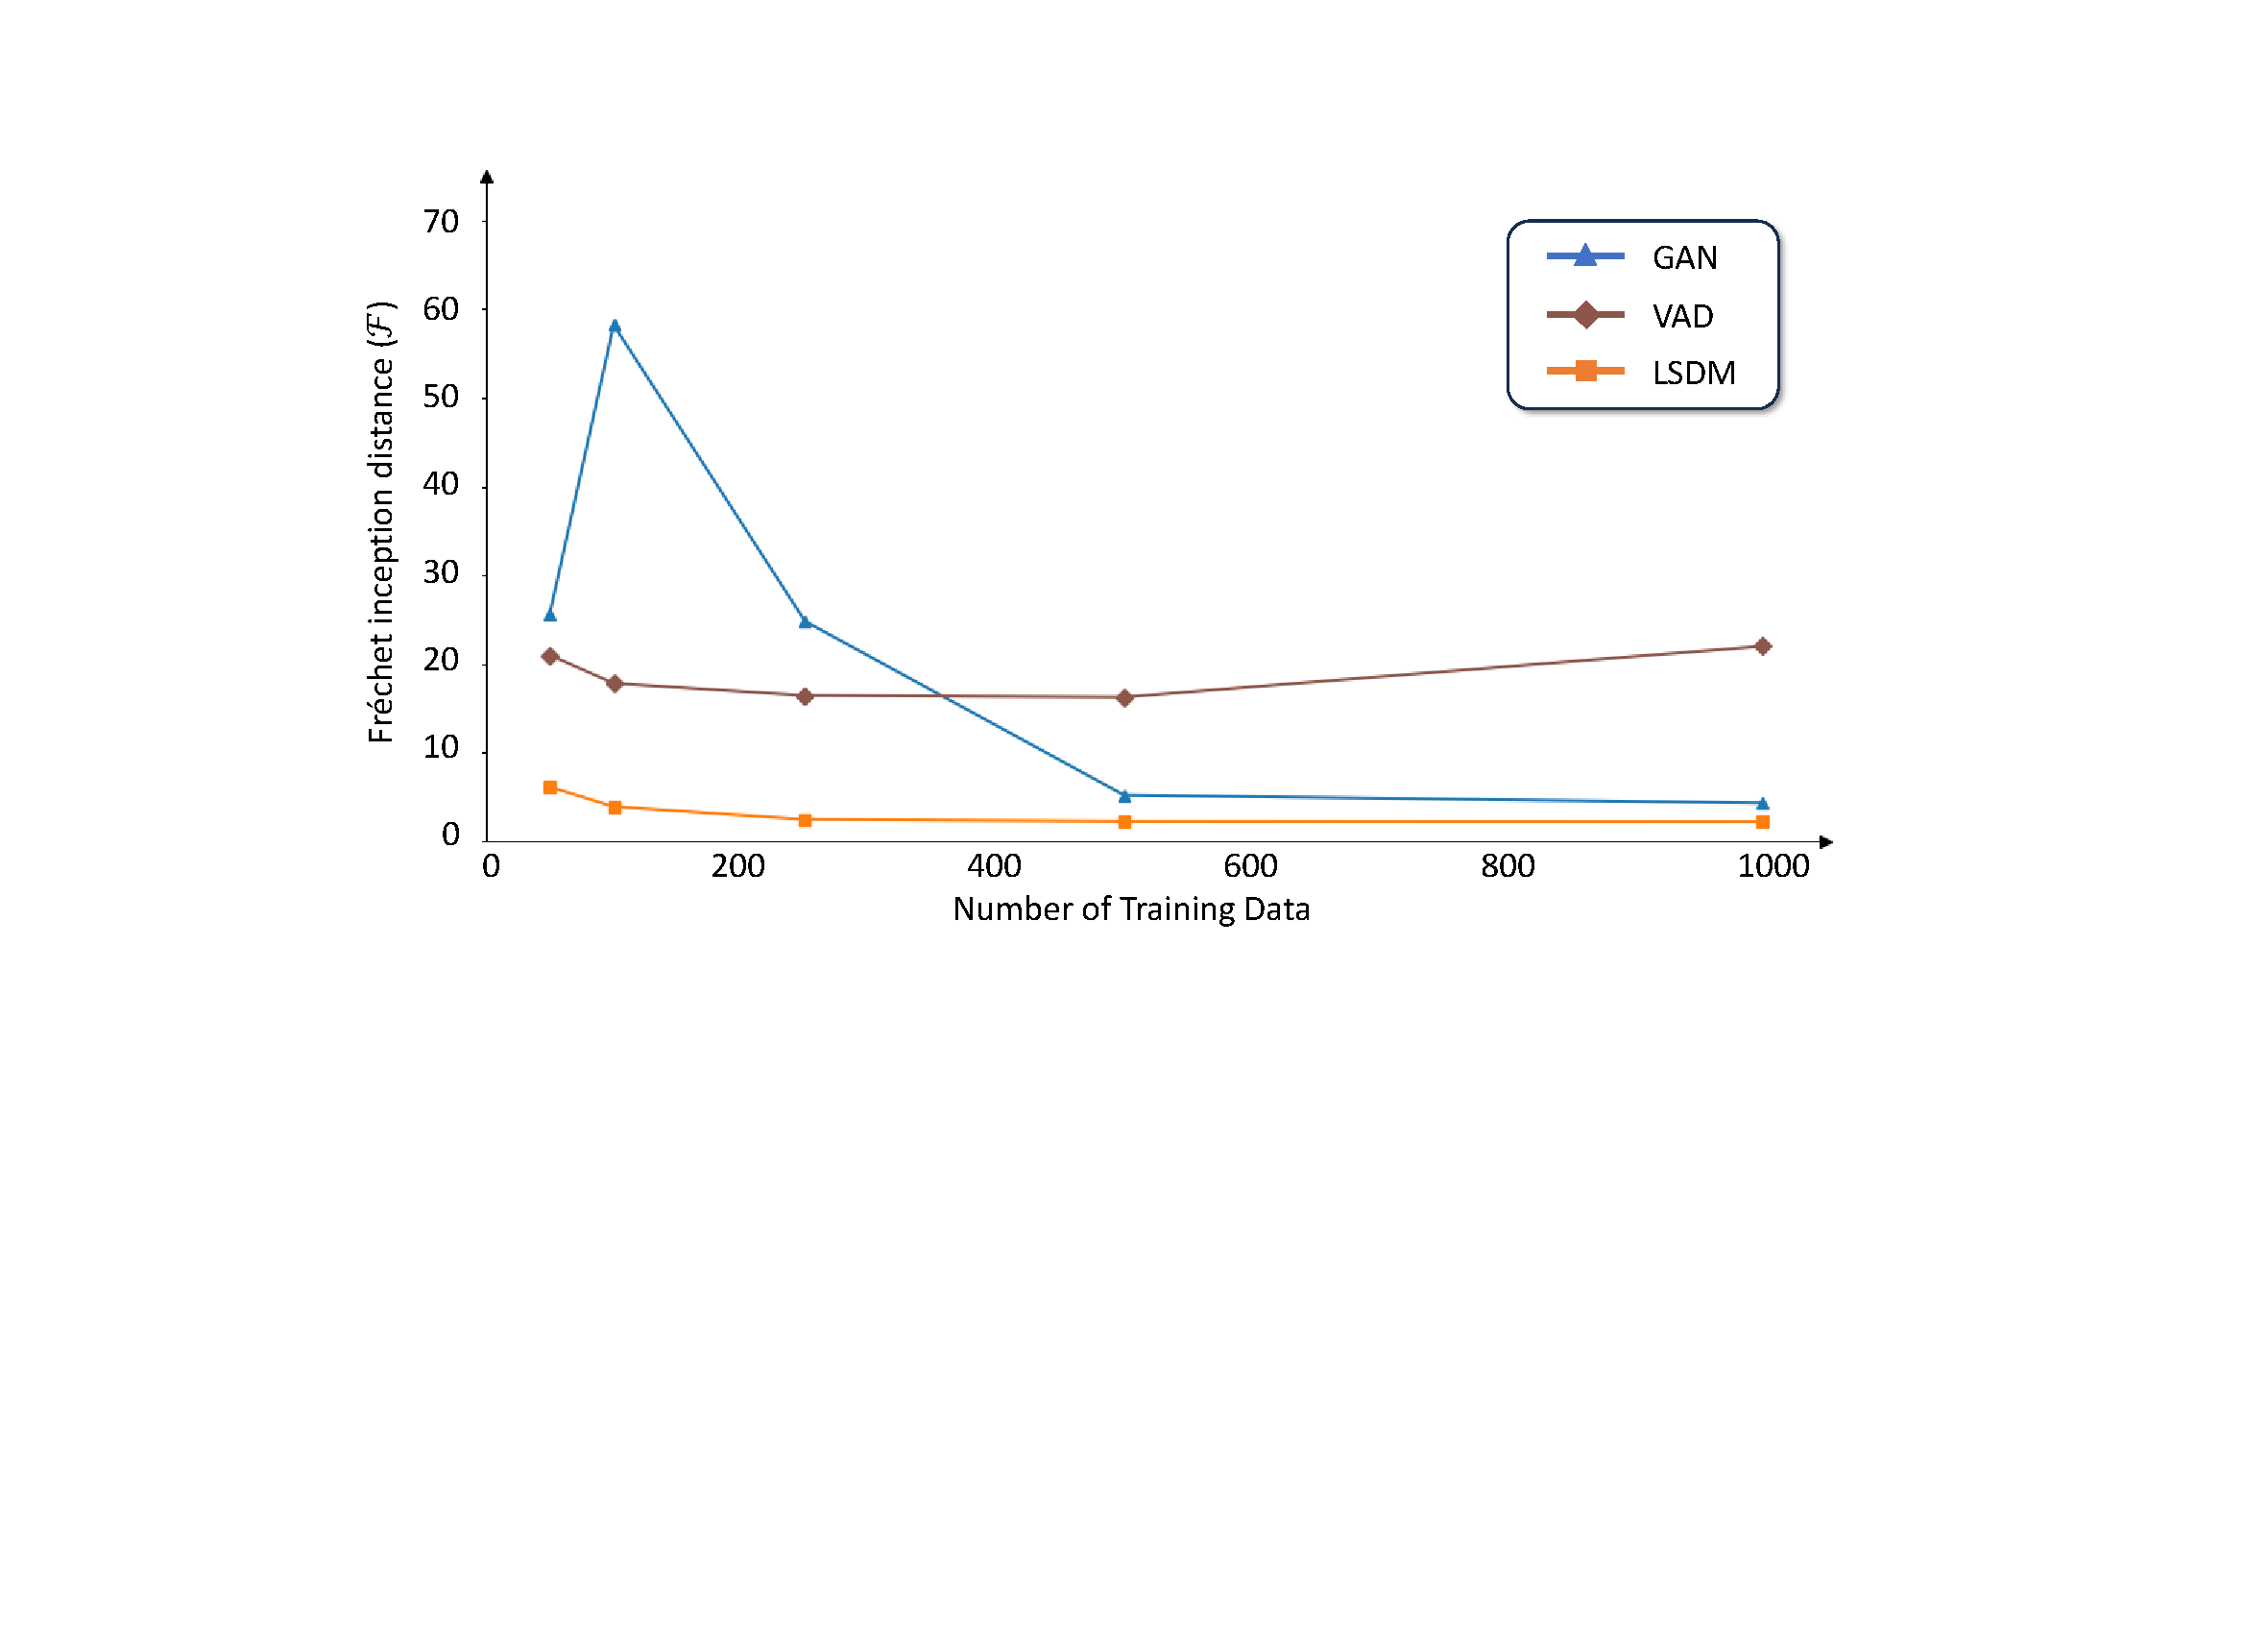
\includegraphics[width=1\linewidth]{chapter6/fig/fig_fid_update.pdf}
    \end{center}
    \vspace{-4mm}
    \caption{
        \small FID scores of airfoils generated by GAN, VAD and LSDM across varying training set sizes. 
    }
    \label{ch6:fig:main_benchmark_fid}
\end{figure}

\subsubsection{Qualitative Comparison}

Fig.~\ref{ch6:fig:main_unconditional_airfoils} provides a visual comparison of airfoils generated by each method (GAN, VAD and LSDM) with progressively smaller training sets. All models produce smooth airfoils with their chords aligned, which reflects the strong geometric prior enforced by the LSM representation. However, there are clear differences in diversity. LSDM generates airfoils with a wide range of shapes with significant variations in thickness distribution, camber, leading-edge radius and position of maximum thickness. This variability still exists even when trained on as few as 50 airfoils. By contrast, GAN suffers from mode collapse given limited data. With fewer than 250 training samples, many GAN outputs collapse to nearly identical shapes and the overall shape variety nearly disappears. VAD does not exhibit catastrophic mode collapse, but its outputs tend to cluster into a few modes. The generated airfoils are less diverse than LSDM’s results and often fall into several families of similar shapes. These qualitative trends indicate that \textit{DiffGeo}’s diffusion-based sampler better preserves shape diversity even under limited data, whereas the GAN struggles and the VAE-style approach produces only moderate diversity.

Fig.\ref{ch6:fig:main_unconditional_tsne} visualizes the latent space coverage of LSDM and GAN using the \textit{t}-Distributed Stochastic Neighbor Embedding algorithm (\textit{t-SNE})~\cite{ai.Maaten2008}. In each subplot, grey points represent latent codes of dataset airfoils from the UIUC database, while orange and blue points represent latent codes generated by LSDM and GAN respectively for different numbers of training data from 1000 down to 50. We can observe that LSDM’s samples closely overlap the distribution of real airfoils in the latent space. Even with very few training shapes, LSDM can still effectively project the multivariate normal prior into LSM's learned manifold, so that the generated latent codes form a similar region as the real data. In contrast, GAN’s samples show significant distributional gaps and clustering. The GAN fails to cover large portions of the latent space that correspond to valid airfoils, and many generated points get clustered, especially given fewer than 250 training samples. These clusters reflect severe mode collapse issues, where GAN produces limited variations. Qualitatively, the \textit{t-SNE} plots demonstrate that LSDM captures the training shape distribution with higher fidelity than the GAN in data-scarce settings. The VAD outputs, though not shown in \textit{t-SNE} due to its probabilistic nature, were observed to generate clear clusters as well, indicating a restricted coverage of the latent space compared to \textit{DiffGeo}.

\subsubsection{Quantitative Evaluation on Sampling Quality}

To quantify how indistinguishable the generated shapes are from the real ones, we compute a Fréchet Inception Distance (FID, denoted as $\cF$) metric with adaptation to aerodynamic shapes. Instead of using an image classifier as in original FID, we use a CFD-based surrogate model trained to predict lift and drag coefficients of airfoils in UIUC database~\cite{aa.Baque2018} to extract feature vectors for each shape. We then calculate FID between the set of generated airfoils and the training dataset in this learned feature space. Given a set of airfoils, feature vectors are inferred from the last hidden layer of the surrogate model. By computing the mean feature vector $\mathcal{M}$ and covariance matrix $\Sigma$, the FID score between two sets of airfoils is defined as:
\begin{equation}
    \cF(\mathcal{M}_1, \mathcal{M}_2, \Sigma_1, \Sigma_2) = \left[ \left|\left| \mathcal{M}_1 - \mathcal{M}_2 \right|\right|^2 + \text{tr}\left( \Sigma_1 + \Sigma_2 - 2\sqrt{\Sigma_1\Sigma_2} \right) \right]^2_F\;.
\end{equation}
To quantify distributional gaps from generated airfoils and training set, $\mathcal{M}_1$ and $\Sigma_1$ are fixed from the UIUC database, while $\mathcal{M}_2$ and $\Sigma_2$ are computed from shapes generated by GAN, VAD and LSDM, respectively.

Fig.~\ref{ch6:fig:main_benchmark_fid} shows the FID scores as a function of training data size. LSDM achieves the lowest and best FID in all cases, indicating its generated airfoils are statistically closest to the distribution of training shapes. With very small training sets (e.g., 50 airfoils), GAN’s FID is much higher, reflecting that GAN outputs deviate significantly from the true data distribution. VAD shows intermediate performance as its FID is higher than LSDM’s but more stable than GAN’s with respect to different dataset. Notably, with larger training sets (e.g., more than 500 samples), GAN’s FID improves and approaches LSDM’s one but LSDM still keeps a slight advantage. In the extreme low-data scenario, LSDM dramatically outperforms GAN while LSDM’s generation fidelity remains largely intact. This highlights \textit{DiffGeo}’s robustness to data scarcity in terms of sample quality.

\begin{figure}[!t]
    \begin{center}
        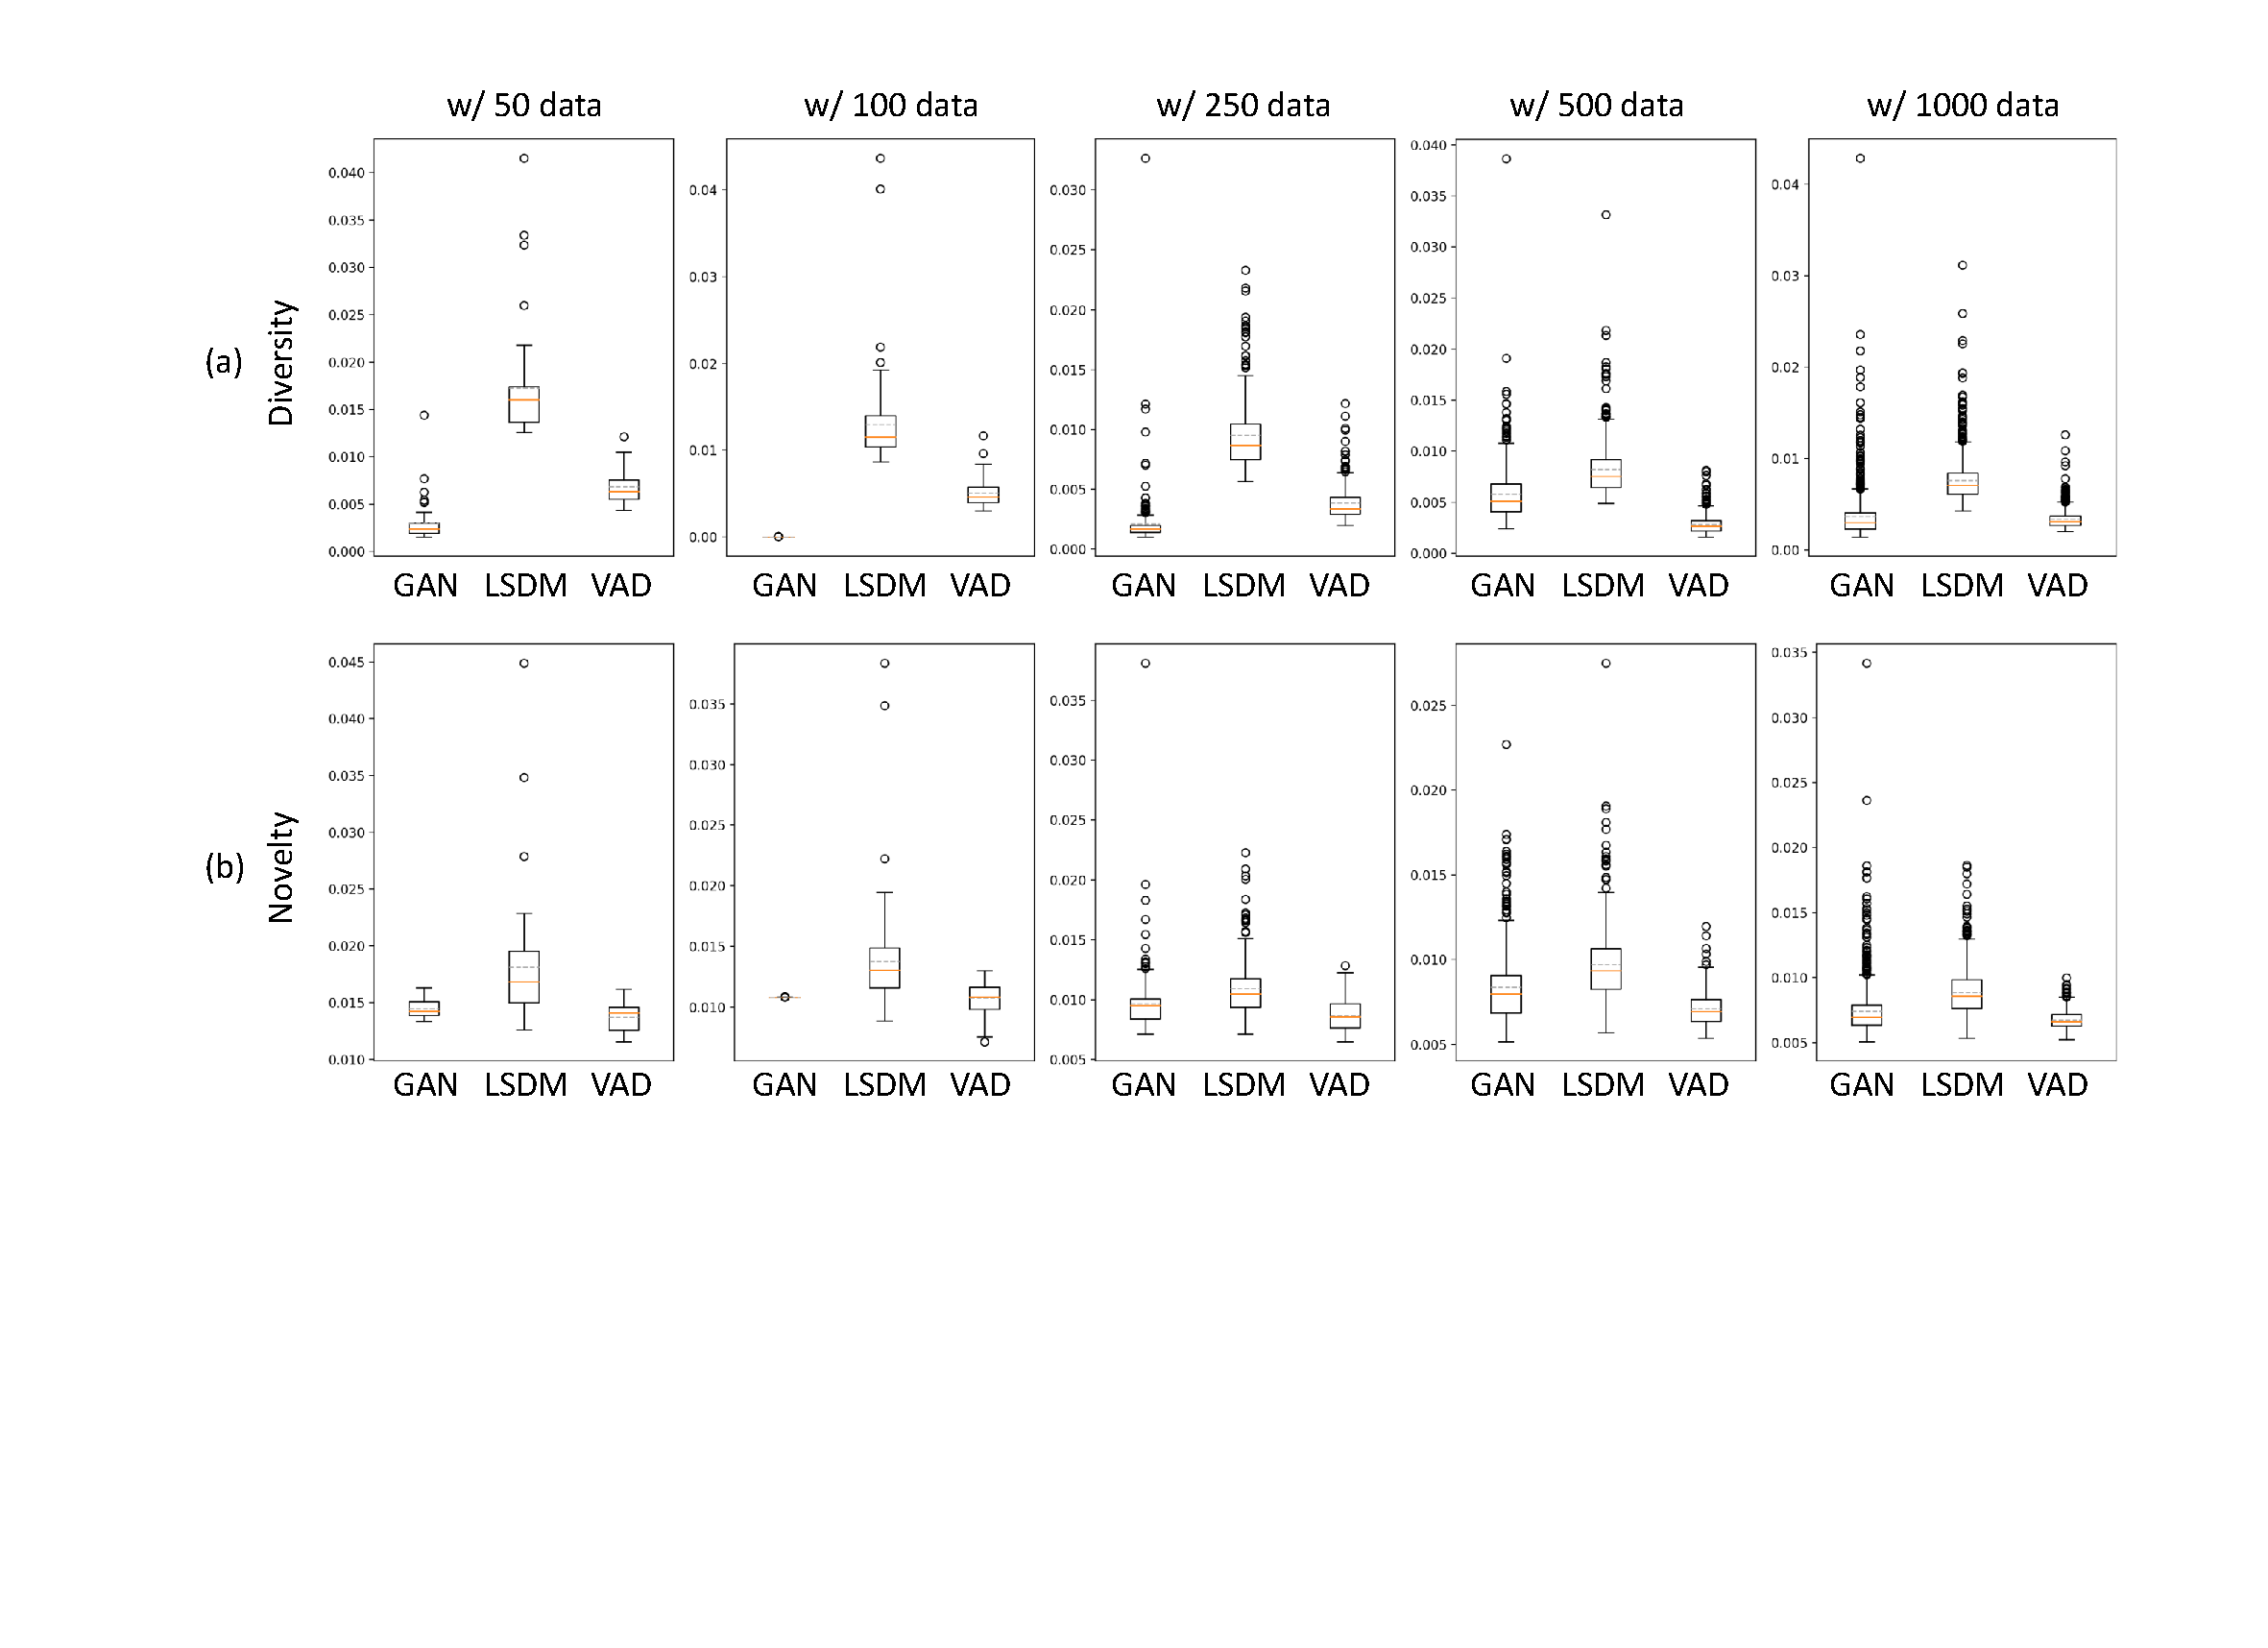
\includegraphics[width=1\linewidth]{chapter6/fig/fig_uncond_inter_intra_dist_updated.pdf}
    \end{center}
    \vspace{-4mm}
    \caption{
        \small Diversity ((a) $D_{intra}^{10}$) and novelty  ((b) $D_{inter}^{10}$) metrics for GAN, VAD and LSDM across dataset sizes. 
    }
    \label{ch6:fig:main_benchmark_unconditional_intra_inter_dist}
\end{figure}

\begin{figure}[!t]
    \begin{center}
        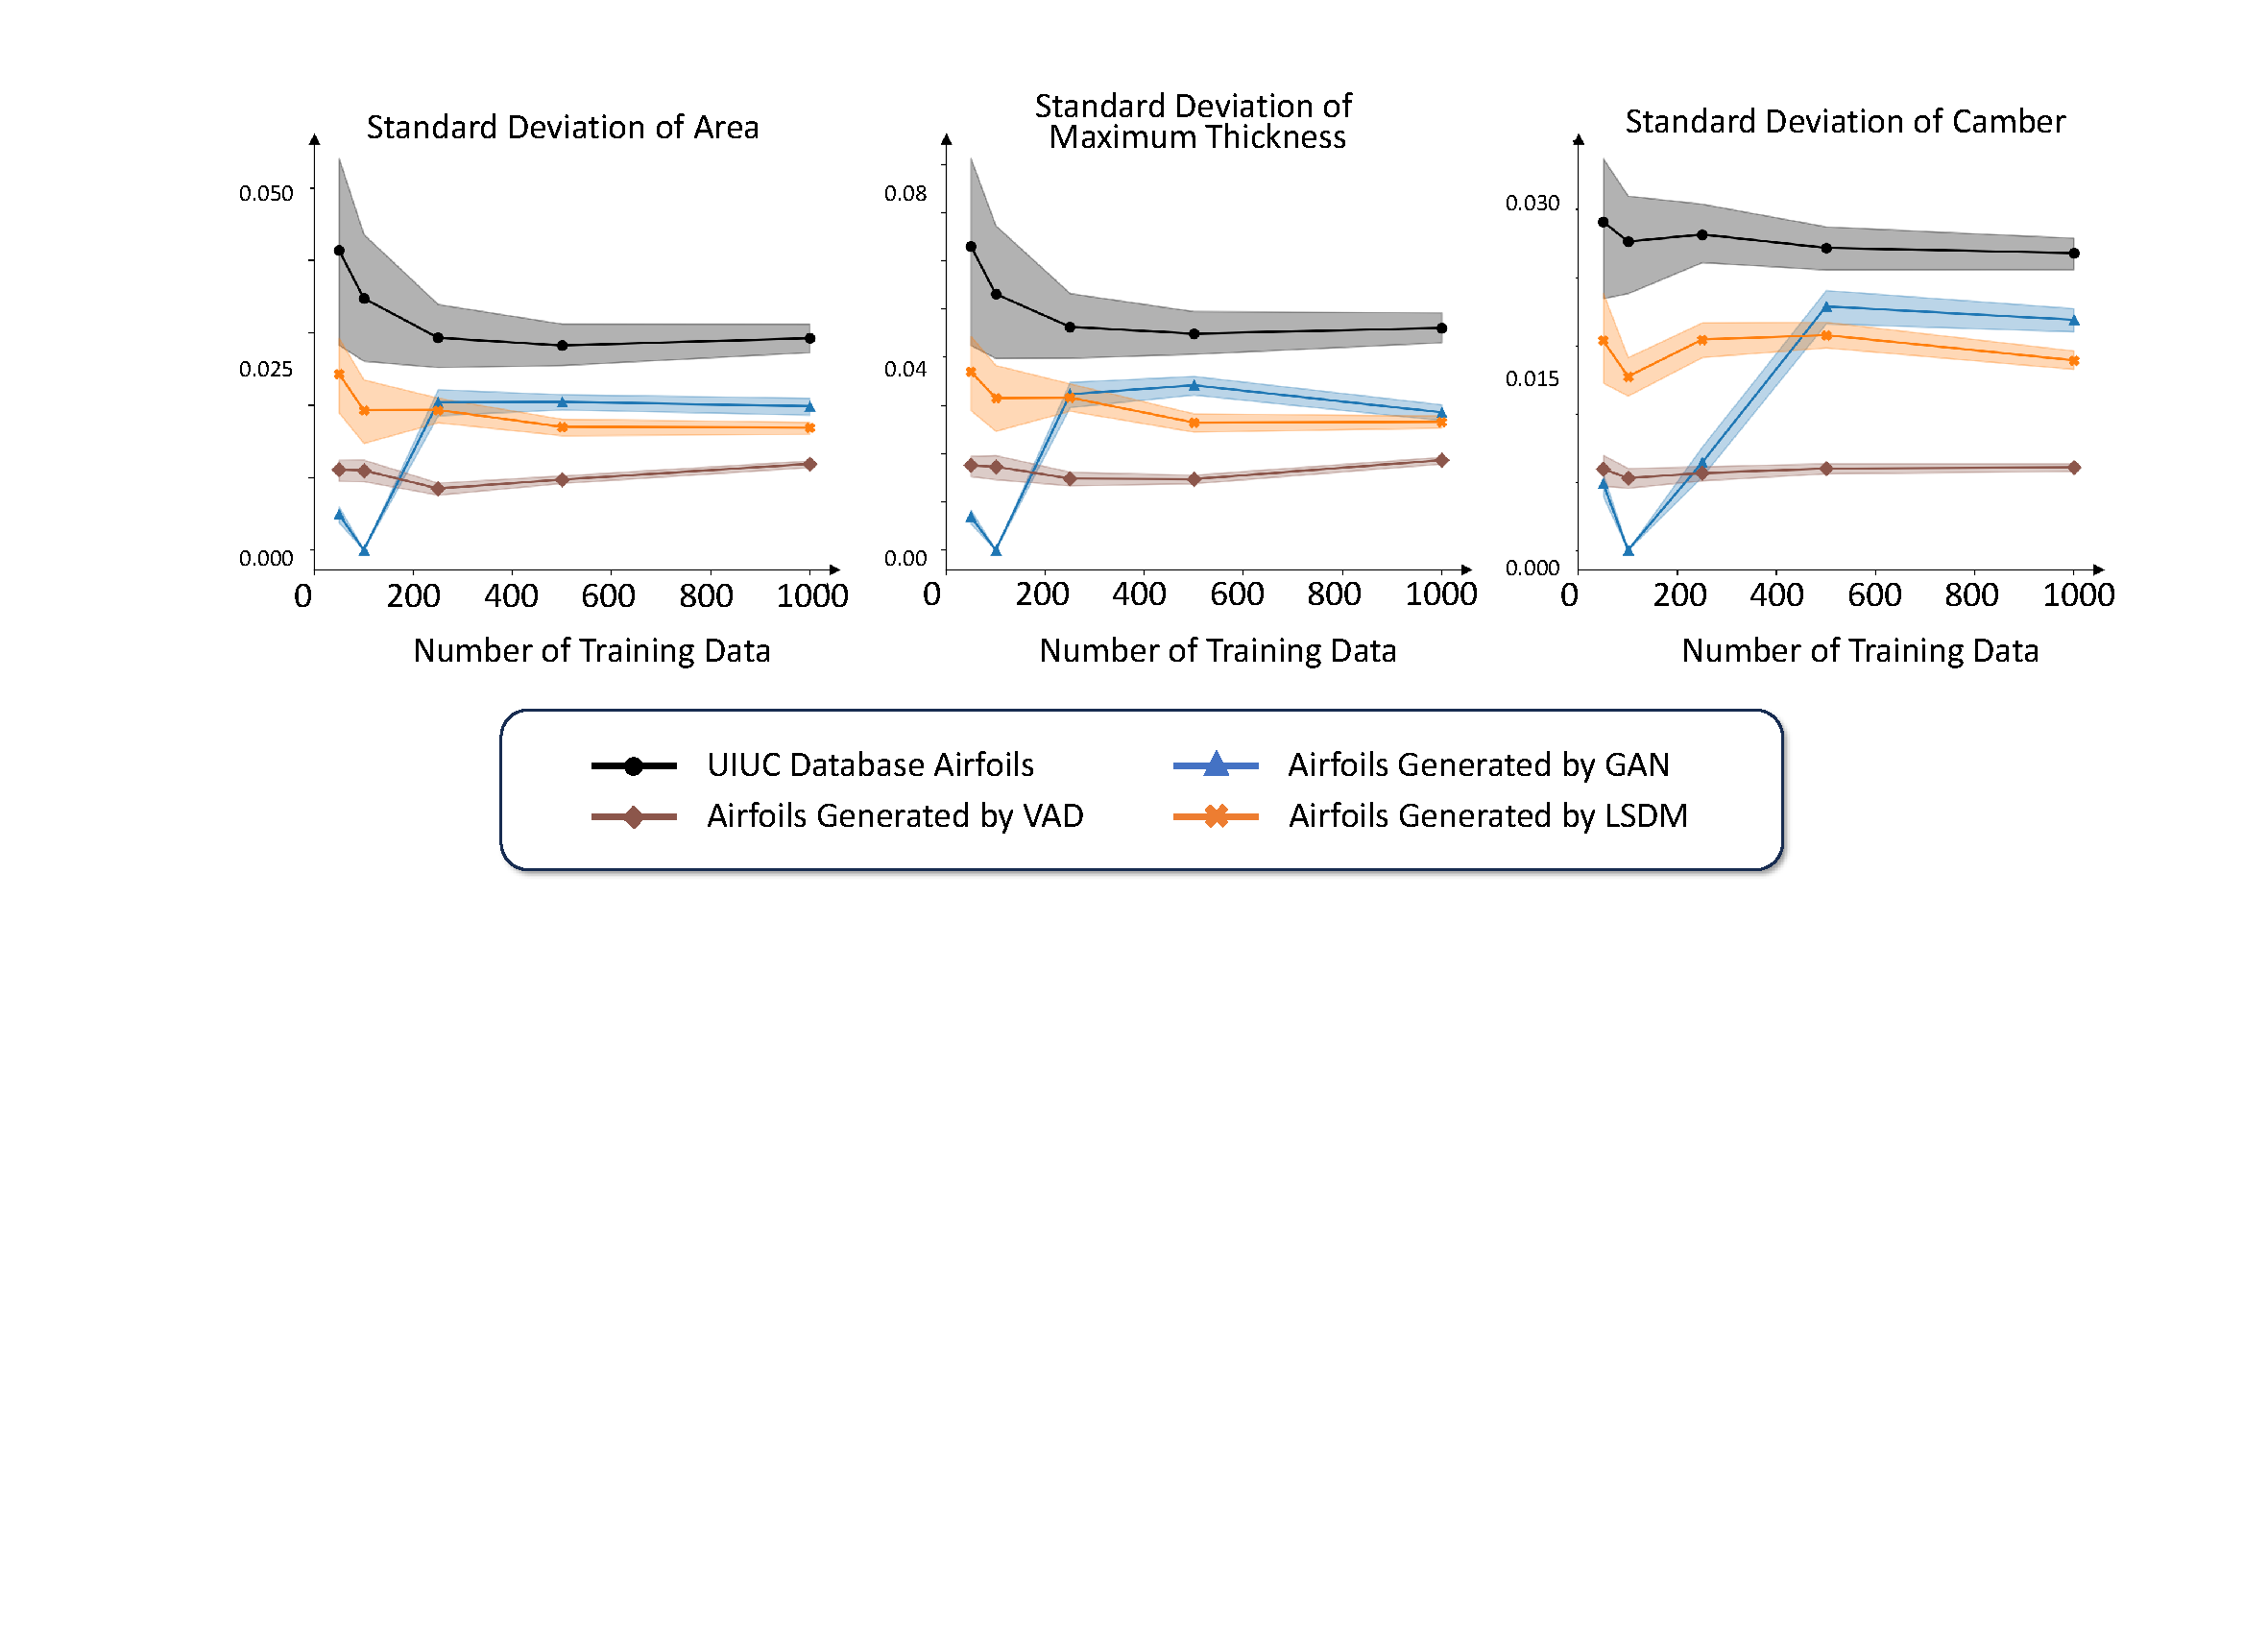
\includegraphics[width=1\linewidth]{chapter6/fig/fig_uncon_std_updated.pdf}
    \end{center}
    \vspace{-2mm}
    \caption{
        \small The standard deviations of area, maximum thickness and camber for GAN, VAD and LSDM. 
    }
    \label{ch6:fig:main_benchmark_unconditional_std}
\end{figure}

\subsubsection{Quantitative Evaluation on Sampling Exploration}

A generative model that successfully explore the design space will generate diverse sets of novel designs. We assess this via two metrics: diversity among generated samples and novelty relative to the training set.

Diversity is a set metric, which measures model's generalization and the information entropy of generated samples. We define a $k$-nearest-intra-sample distance $D_{intra}^k$ to measure diversity. For each newly generated airfoil, we compute the average chamfer distance (CD) to its $k=10$ nearest neighbors within the generated set, then take the mean over all generated samples. A higher $D_{intra}^{10}$ means the set of outputs covers a broader range of shapes and have higher variability.

Novelty is a point metric that measures how far generated shapes deviate from real designs in the training set. Similarly, we define a $k$-nearest-inter-sample distance $D_{inter}^k$ as the average distance from each generated airfoil to its $k=10$ nearest neighbors in the training dataset. Higher values indicate the generator is producing shapes that are different from those in the training set while still remaining valid designs.

Fig.~\ref{ch6:fig:main_benchmark_unconditional_intra_inter_dist} demonstrates the computed $D_{intra}^{10}$ and $D_{inter}^{10}$ for GAN, VAD and LSDM under various training set sizes. LSDM has the highest scores in both diversity and novelty across all scenarios. With sufficient data (e.g., 1000 samples), all methods achieve certain diversity, but LSDM is still above GAN and VAD. As training data reduced, GAN’s diversity and novelty collapse. For example, with 100 or 50 samples, GAN-generated airfoils show almost no diversity where $D_{intra}^{10}$ is close to zero and very low novelty, meaning that the few representative shapes GAN can generate are clustered near some training examples. VAD maintains a more consistent diversity and novelty level regardless of data size without any catastrophic mode collapse, but its absolute values are lower than LSDM in every case. In comparison, LSDM remains high diversity and novelty even with only 50 training airfoils and is not affected by data scarcity.

\begin{figure}[!th]
    \begin{center}
        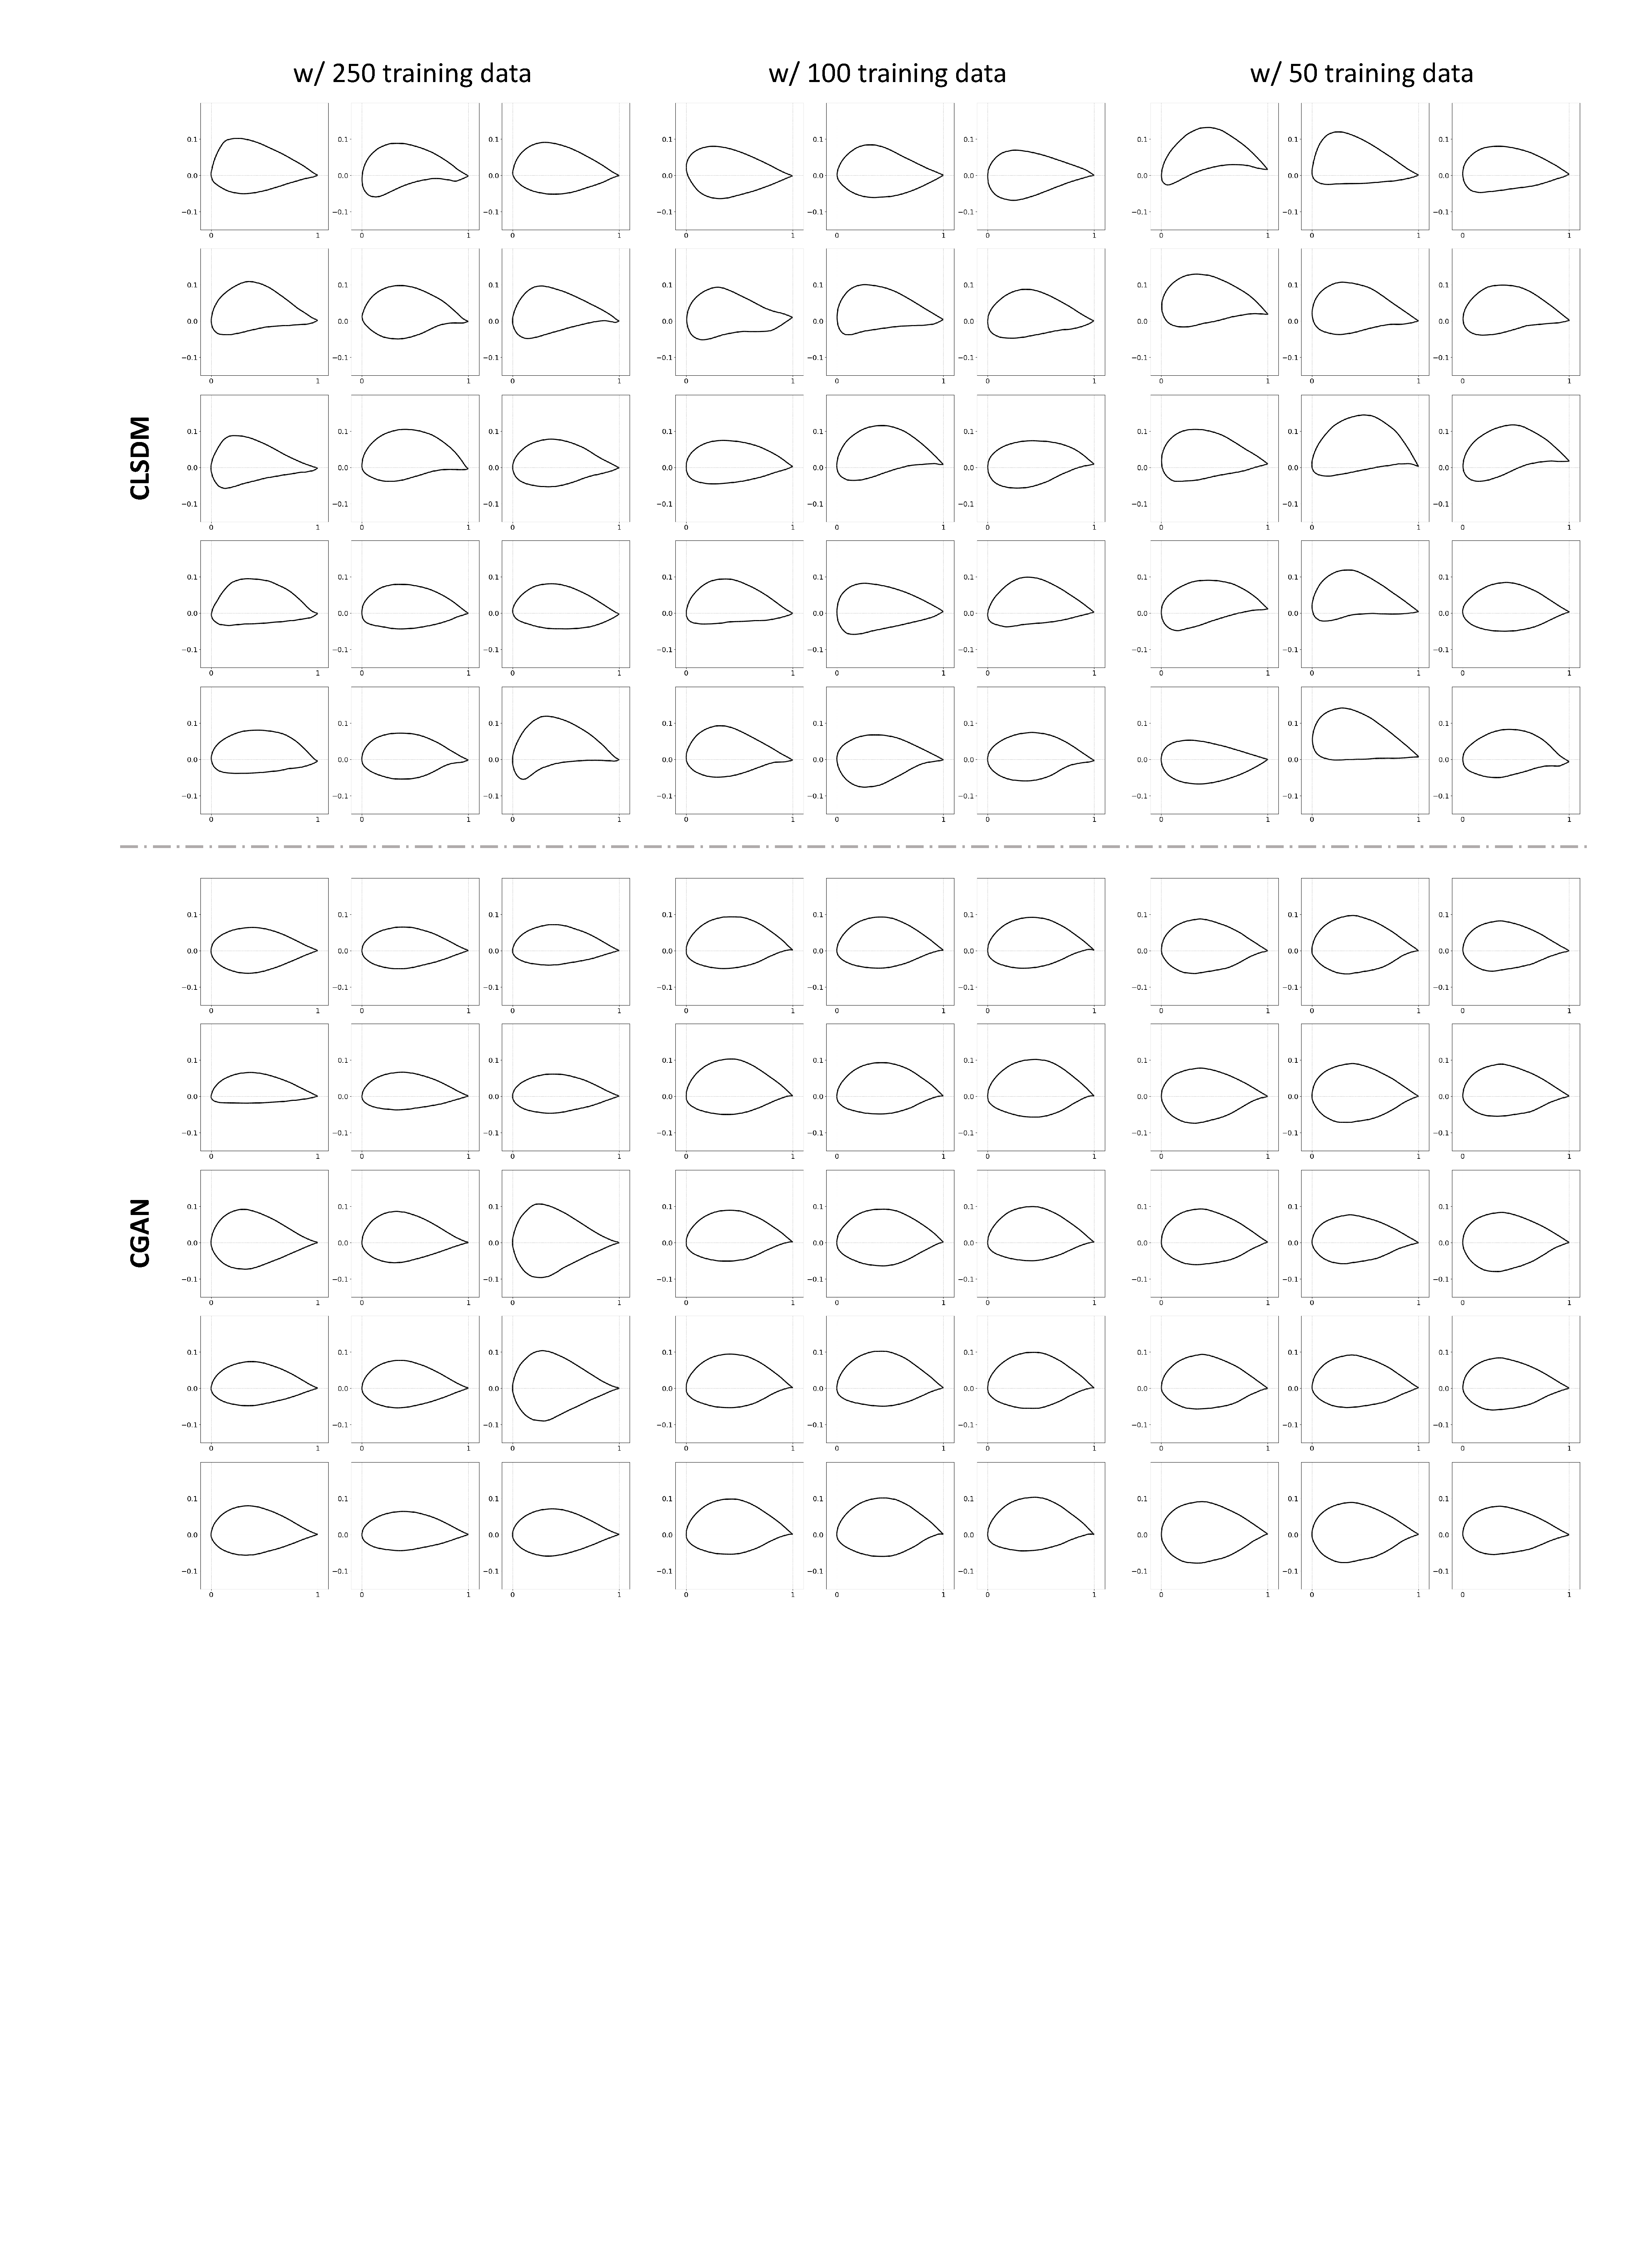
\includegraphics[width=1\linewidth]{chapter6/fig/fig_con_airfoils_updated.pdf}
    \end{center}
    \caption{
     \small Airfoils conditioned on $\mathcal{A}=0.09$ sampled by CLSDM and CGAN.
    }
    \label{ch6:fig:main_conditional_airfoils}
\end{figure}

We also directly measured the distribution of specific geometric properties among generated samples as shown in Fig.~\ref{ch6:fig:main_benchmark_unconditional_std}, including the standard deviations of airfoil area, maximum thickness and camber for each model. Consistent with the $D_{intra}^{10}$ metric, LSDM and VAD exhibit relatively flat variance curves as the number of training data varies, indicating they continue to produce a certain range of shapes. In contrast, GAN’s output variability drops with fewer than 200 training shapes. For very low data settings, GAN’s generated airfoils all have nearly the same area/thickness/camber, leading to negligible standard deviations that reflect severe mode collapse. VAD’s variance is more stable but is uniformly lower than that of LSDM, meaning that LSDM explores a wider range of geometries.

\subsubsection{Discussion}

In summary, the benchmark results demonstrate that \textit{DiffGeo}’s diffusion-based sampler LSDM consistently outperforms GAN- and VAE-based approaches in both sampling quality and sampling exploration, especially under low-data settings. Compared to adversarial training, LSDM offers stable generation without mode collapse, eliminating the need for large training sets or extensive hyperparameter tuning to stabilize GANs. Compared to the variational and prior-based sampling strategy, LSDM leverages the full representation capacity of the auto-decoder, which VAEs often compromise due to its regularization. As a result, LSDM produces more diverse and higher-fidelity samples. Although VAE and VAD can avoid mode collapse, their performance is degraded by a less expressive latent representation. In summary, for the unconditional generation task, \textit{DiffGeo} achieves nearly an order-of-magnitude improvement in data efficiency over GANs and shows clear advantages over VAD in diversity and novelty. These findings answer the first two comparison points: diffusion-based sampling performs better than adversarial training in stability, and than a fixed latent prior in flexibility and output quality.

\subsubsection{Conditional Generation Benchmark}
In this section,  we evaluate conditional generative performance by comparing the conditional LSDM (CLSDM) against conditional GAN (CGAN). This investigation addresses how well each approach can integrate design constraints into the generation process, especially with limited data. For a concrete comparison, we choose a simple conditioning objective, namely generating airfoils that satisfy a constant area value (e.g., $0.09$ for this case). The CGAN is retrained to model a joint probability of data and condition for each dataset size with area as the conditioning input, while CLSDM uses energy-based guidance to enforce the area during sampling without any additional training. 

To investigate conditional generation quality, we sample a large number of airfoils from each model under the condition of area being $0.09$. For CLSDM, we implement Equation~\ref{ch6:eq:energy_guidance} with the equality constraint $C^E$ that uses the closed-form Shoelace Formula to calculate the area $\mathcal{A}$. Given vertices on airfoil's contour in clockwise or anti-clockwise order $V=\{\bv_1, \bv_2,...\bv_N\}$, $\mathcal{A}$ is defined as:
\begin{equation}
    \mathcal{A}(V) = \frac{1}{2} \sum_{i=1}^N \left(v_{i,x}v_{i+1,y} - v_{i+1,x}v_{i,y} \right)\;,\;\text{where}\;\bv_i = (v_{i,x},v_{i,y})\;.
\end{equation}
Then we have $C^E = \bigl\| \mathcal{A}(V)-0.09\bigr\| ^2$. For CGAN, its input condition remains a constant scalar as $C=0.09$.

\begin{figure}[!t]
    \vspace{-6mm}
    \begin{center}
        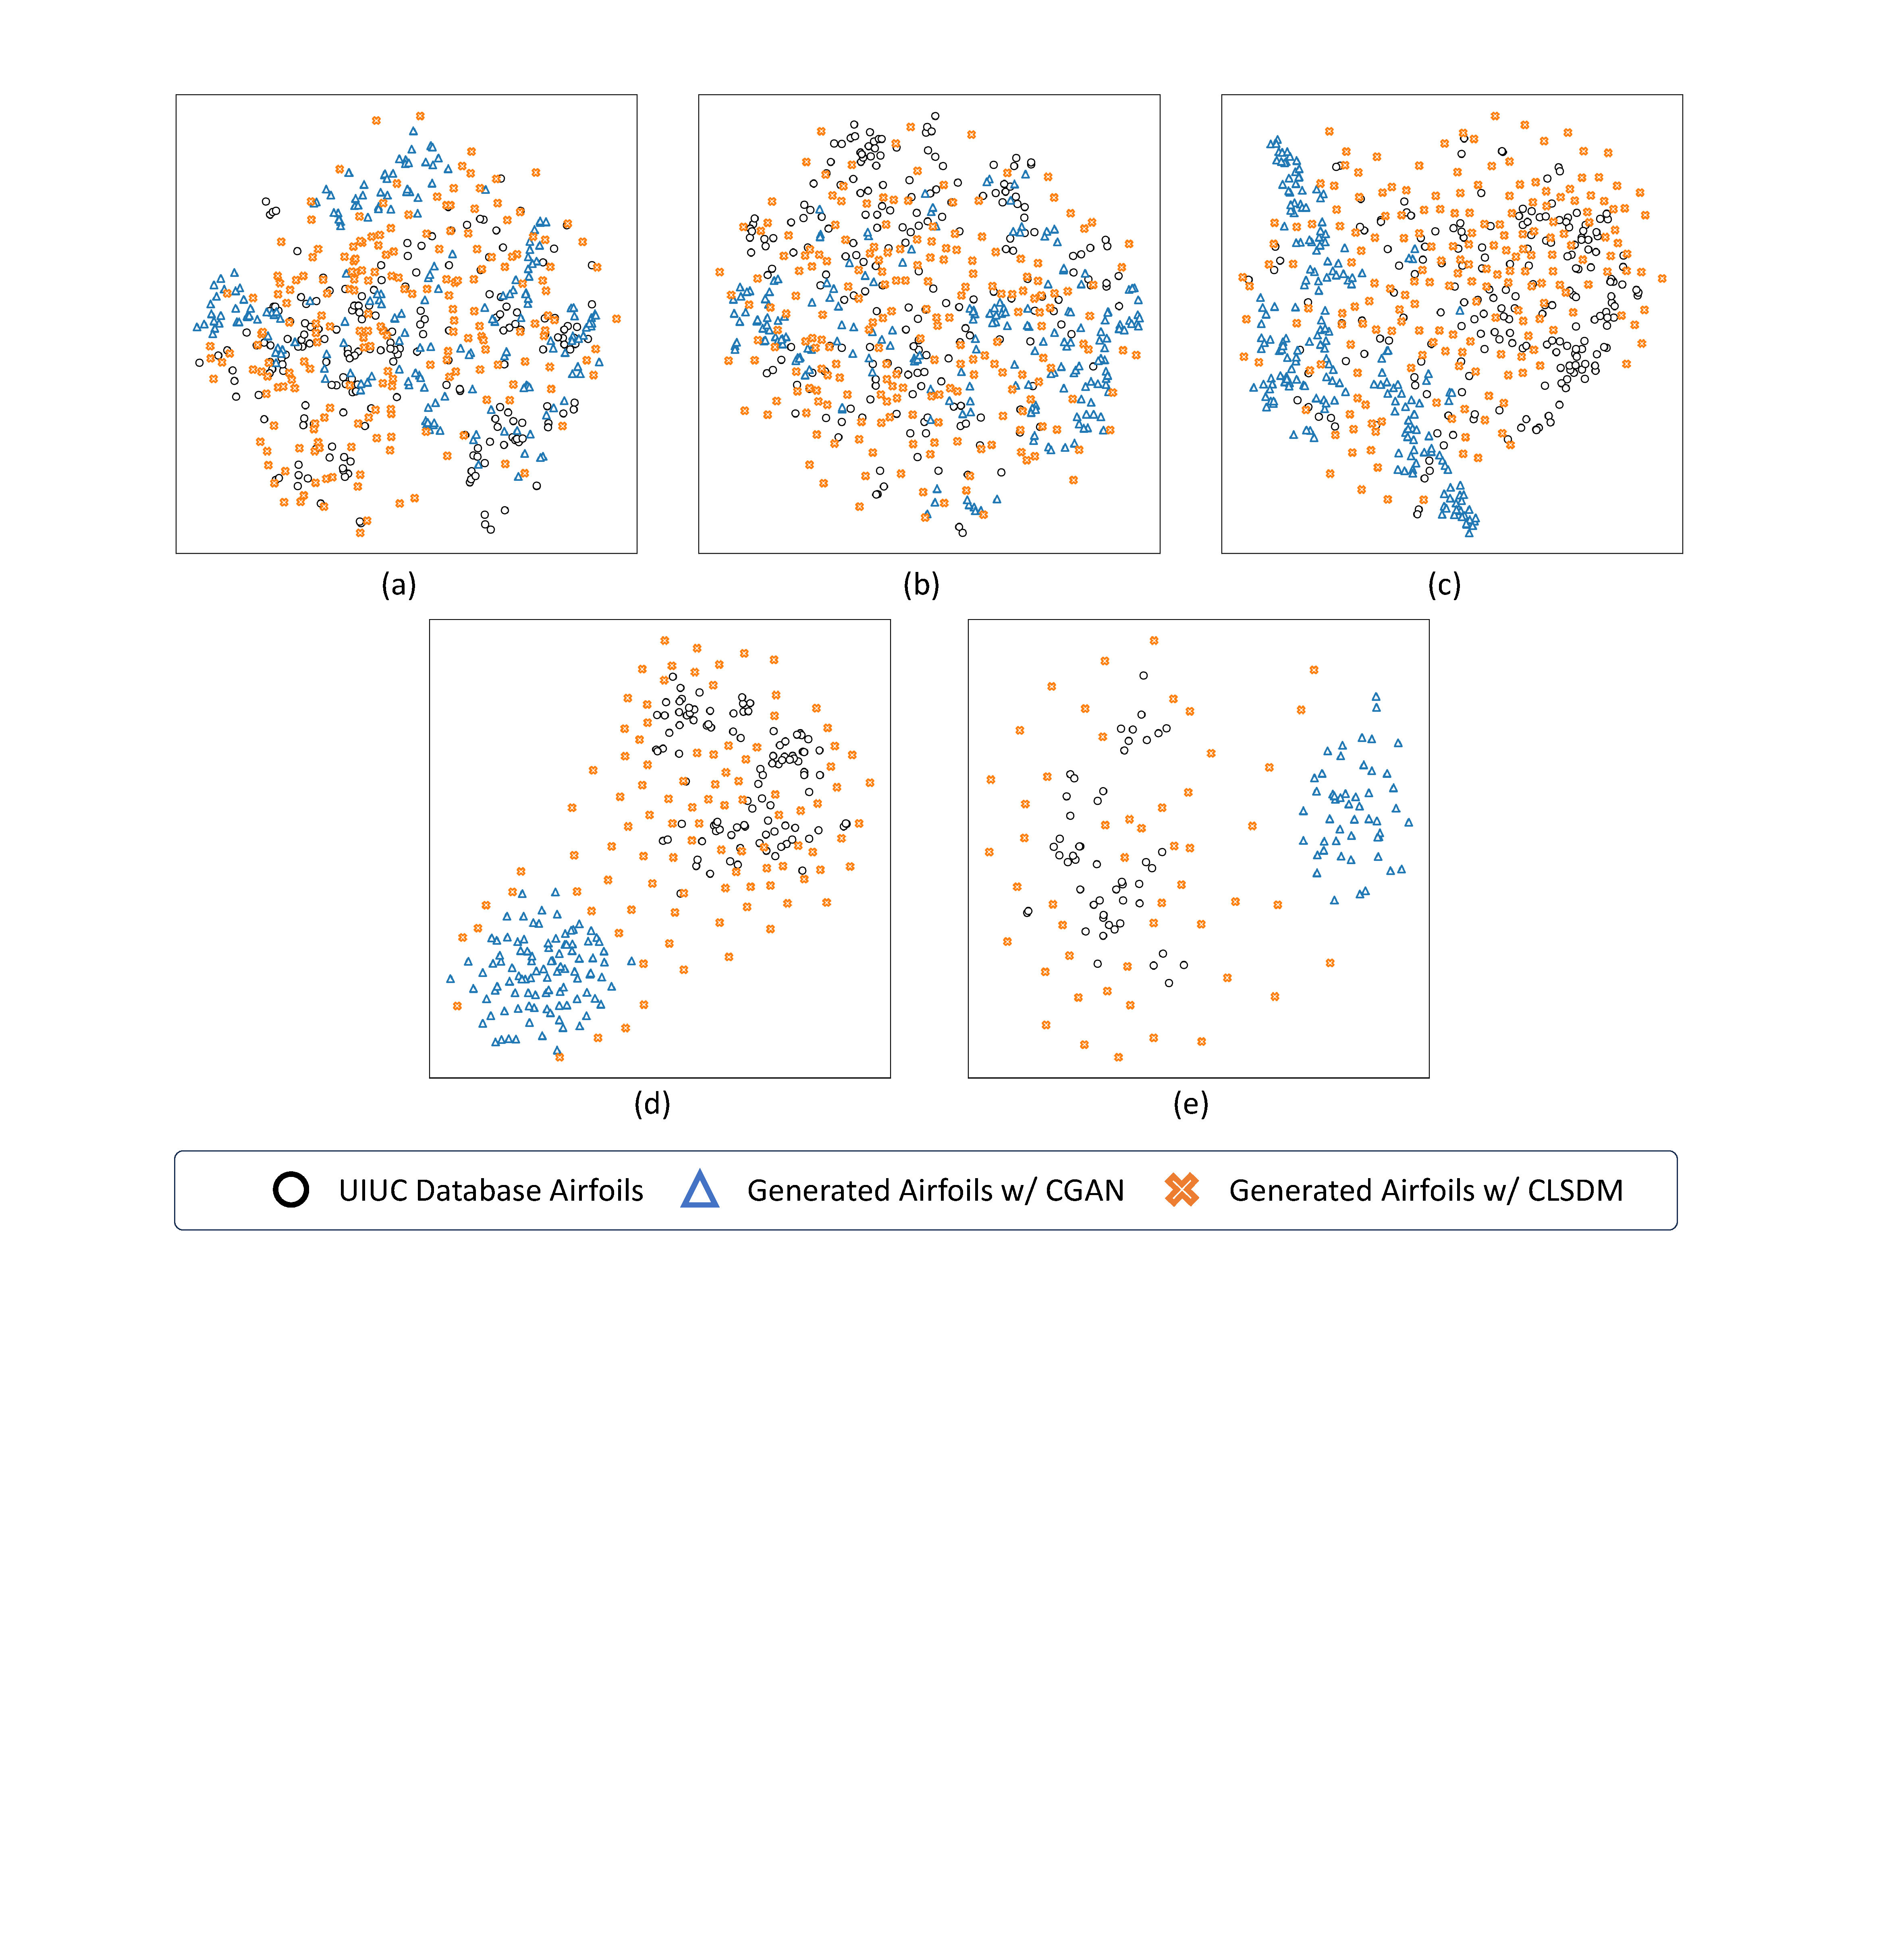
\includegraphics[width=0.9\linewidth]{chapter6/fig/conditional_tsne.pdf}
    \end{center}
    \vspace{-4mm}
    \caption{
        \small \textit{t-SNE} visualization of airfoils' latent codes from UIUC database, CLSDM and CGAN under $\mathcal{A}=0.09$ for training sizes of (a) $1000$, (b) $500$, (c) $250$, (d) $100$ and (e) $50$ airfoils.
    }
    \label{ch6:fig:main_conditional_tsne}
\end{figure}

Fig.~\ref{ch6:fig:main_conditional_airfoils} shows generated airfoils sampled by CLSDM and CGAN. Similar as the conclusion draw from the unconditional generation benchmark, all samples exhibit valid airfoil properties, and CLSDM consistently demonstrates better diversity than CGAN, especially with fewer than 250 training data. Although airfoils sampled by CGAN trained with 250 samples show more variety, the area condition is not always respected, as can be observed in Fig.~\ref{ch6:fig:main_conditional_airfoils}(d). Fig.~\ref{ch6:fig:main_conditional_tsne} provides the \textit{t-SNE} visualization in the latent space. CLSDM aligns better with the training data distribution while CGAN's distributions are clearly biased and clustered, showing CGAN's poorer sampling quality and diversity compared to CLSDM.

The condition adherence performance is measured by the difference between each generated airfoil’s actual area and the target value. Fig.~\ref{ch6:fig:main_benchmark_condition_mae_boxplot} plots the mean absolute error in area for CGAN and CLSDM at various training set sizes. CLSDM shows significantly lower error, indicating that \textit{DiffGeo} is able to satisfy the target area closely for its samples even with very few training data. Meanwhile, CGAN struggles to enforce the area constraint since its error is an order of magnitude higher and does not improve by a large margin with more data. This indicates that energy-based diffusion guidance is far more effective at satisfying constraints than the GAN’s learned conditioning, especially since the GAN must implicitly learn the mapping from condition to shape during training which is difficult with limited data and a single scalar condition.

\begin{figure}[!t]
    \begin{center}
        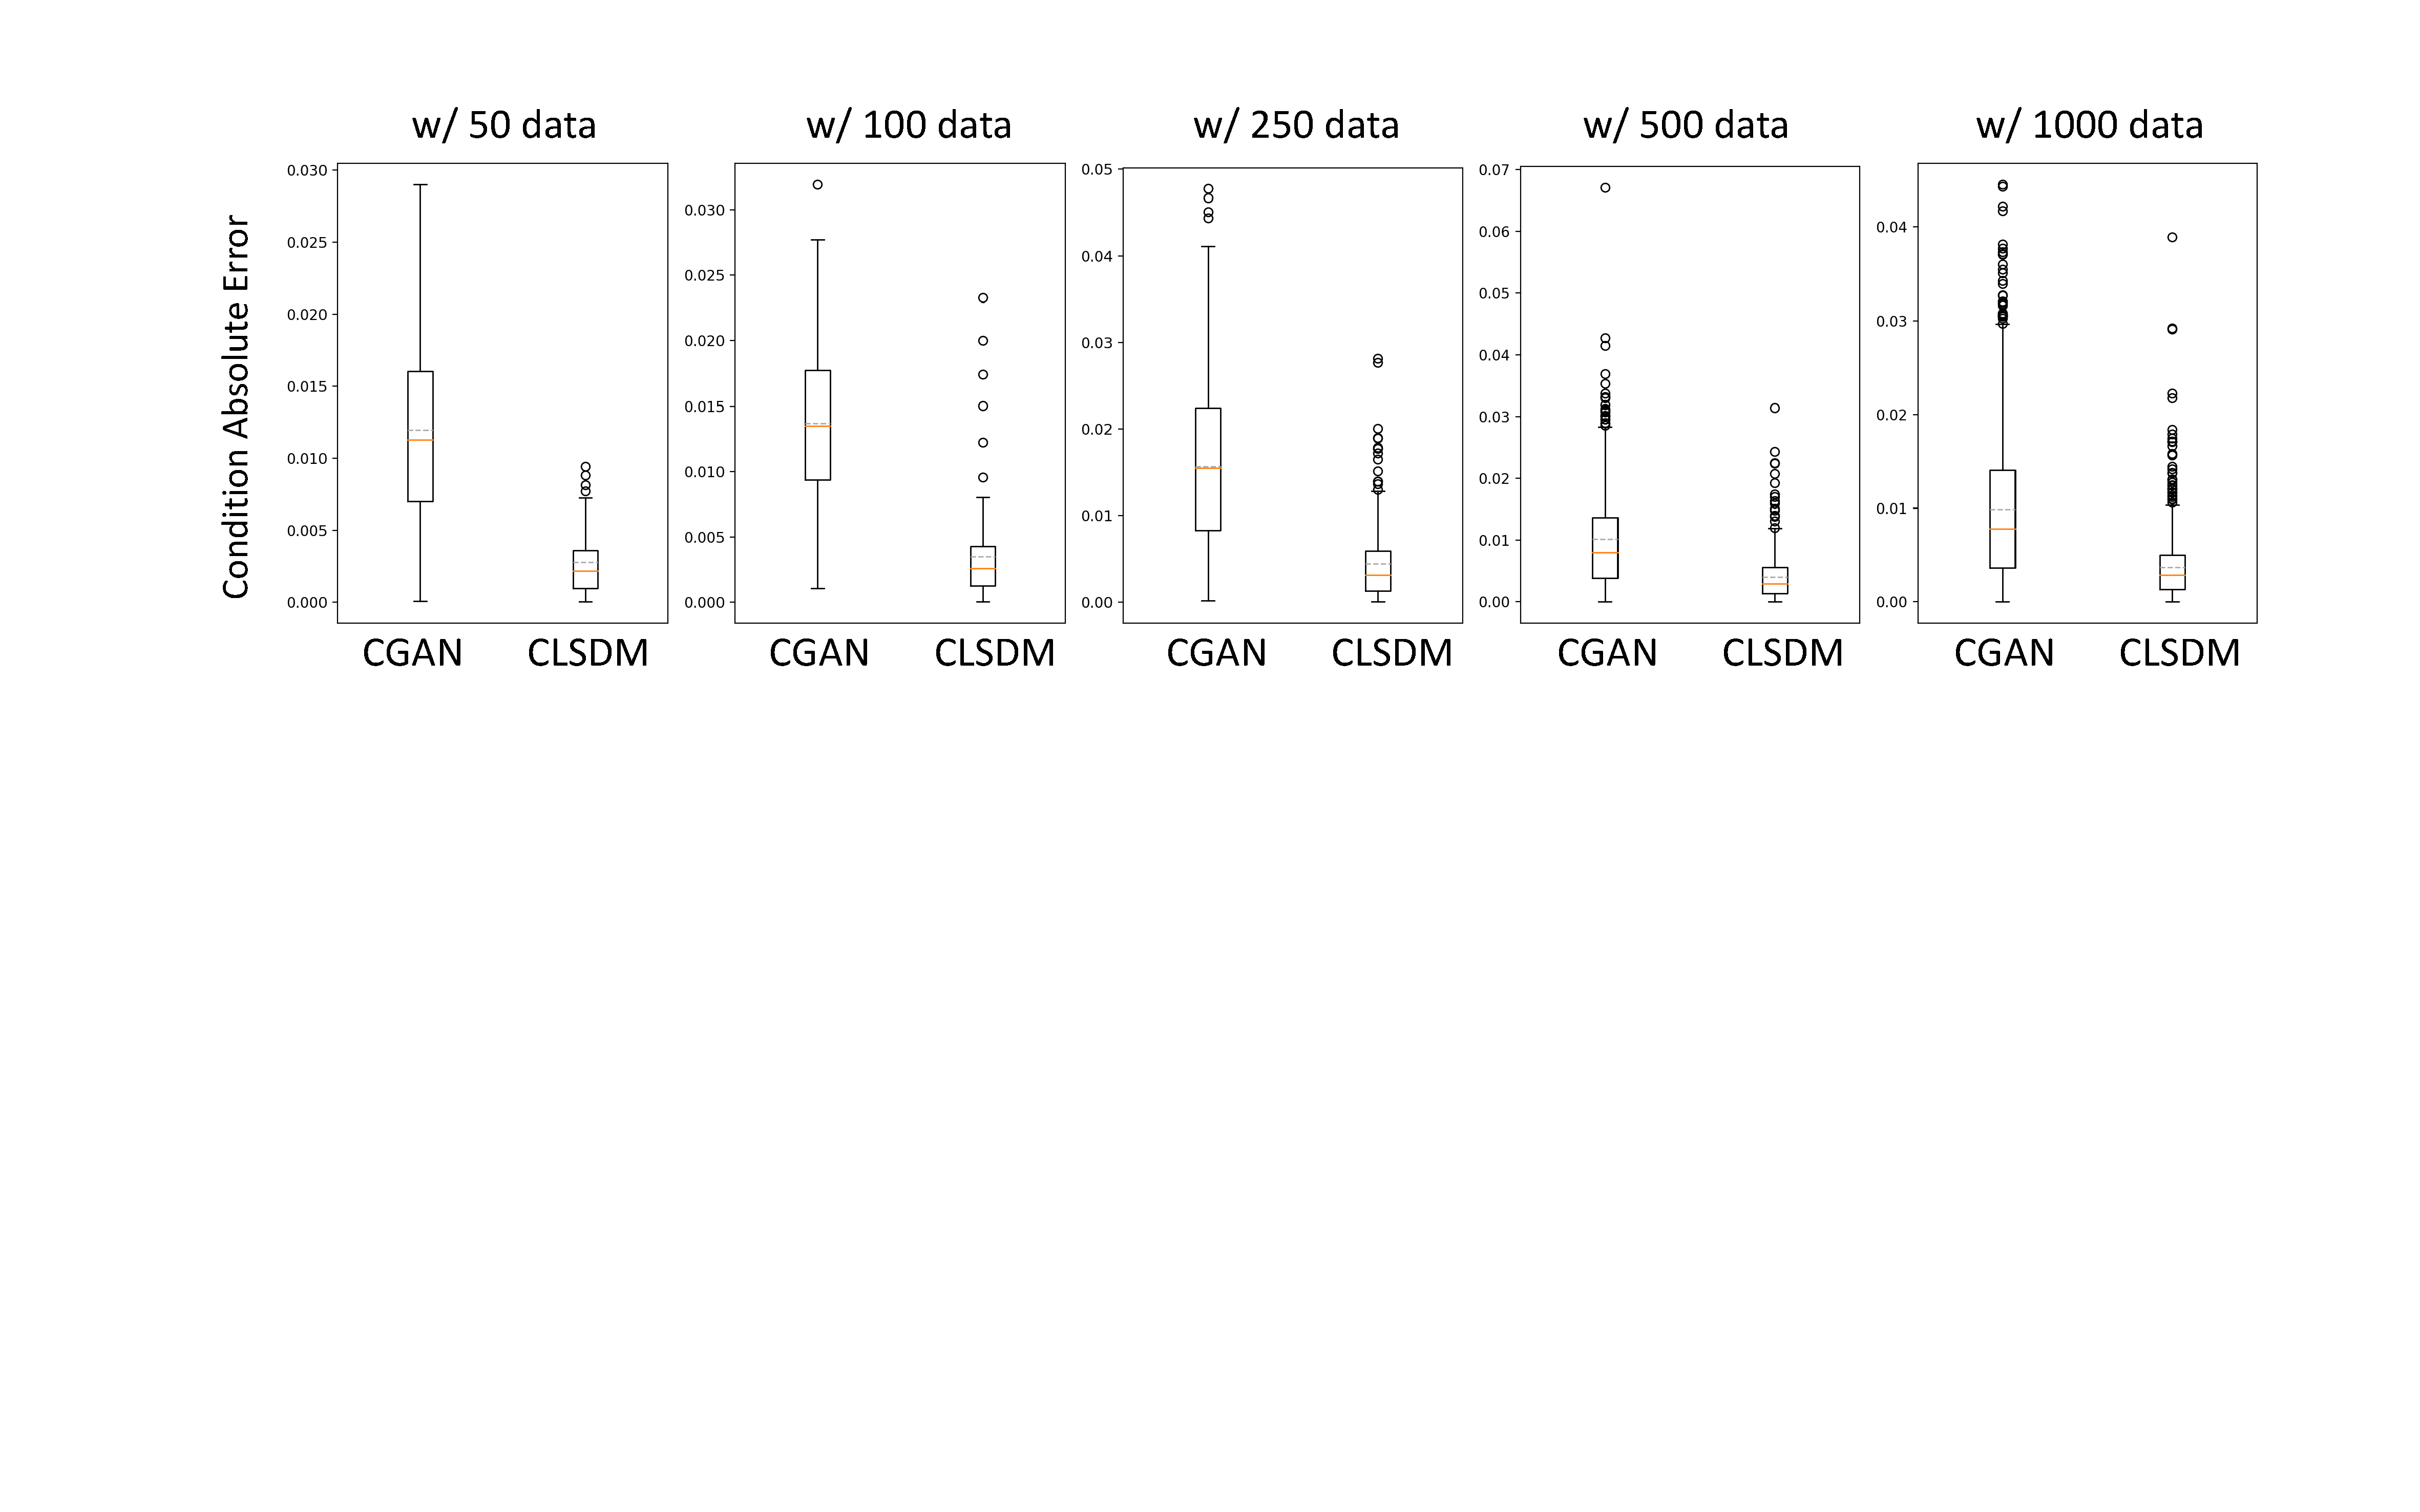
\includegraphics[width=1\linewidth]{chapter6/fig/condition_mae_box_plot.pdf}
    \end{center}
    \vspace{-2mm}
    \caption{
        \small Mean absolute area error of CLSDM and CGAN conditioned airfoils.
    }
    \label{ch6:fig:main_benchmark_condition_mae_boxplot}
\end{figure}

\begin{figure}[!ht]
    \begin{center}
        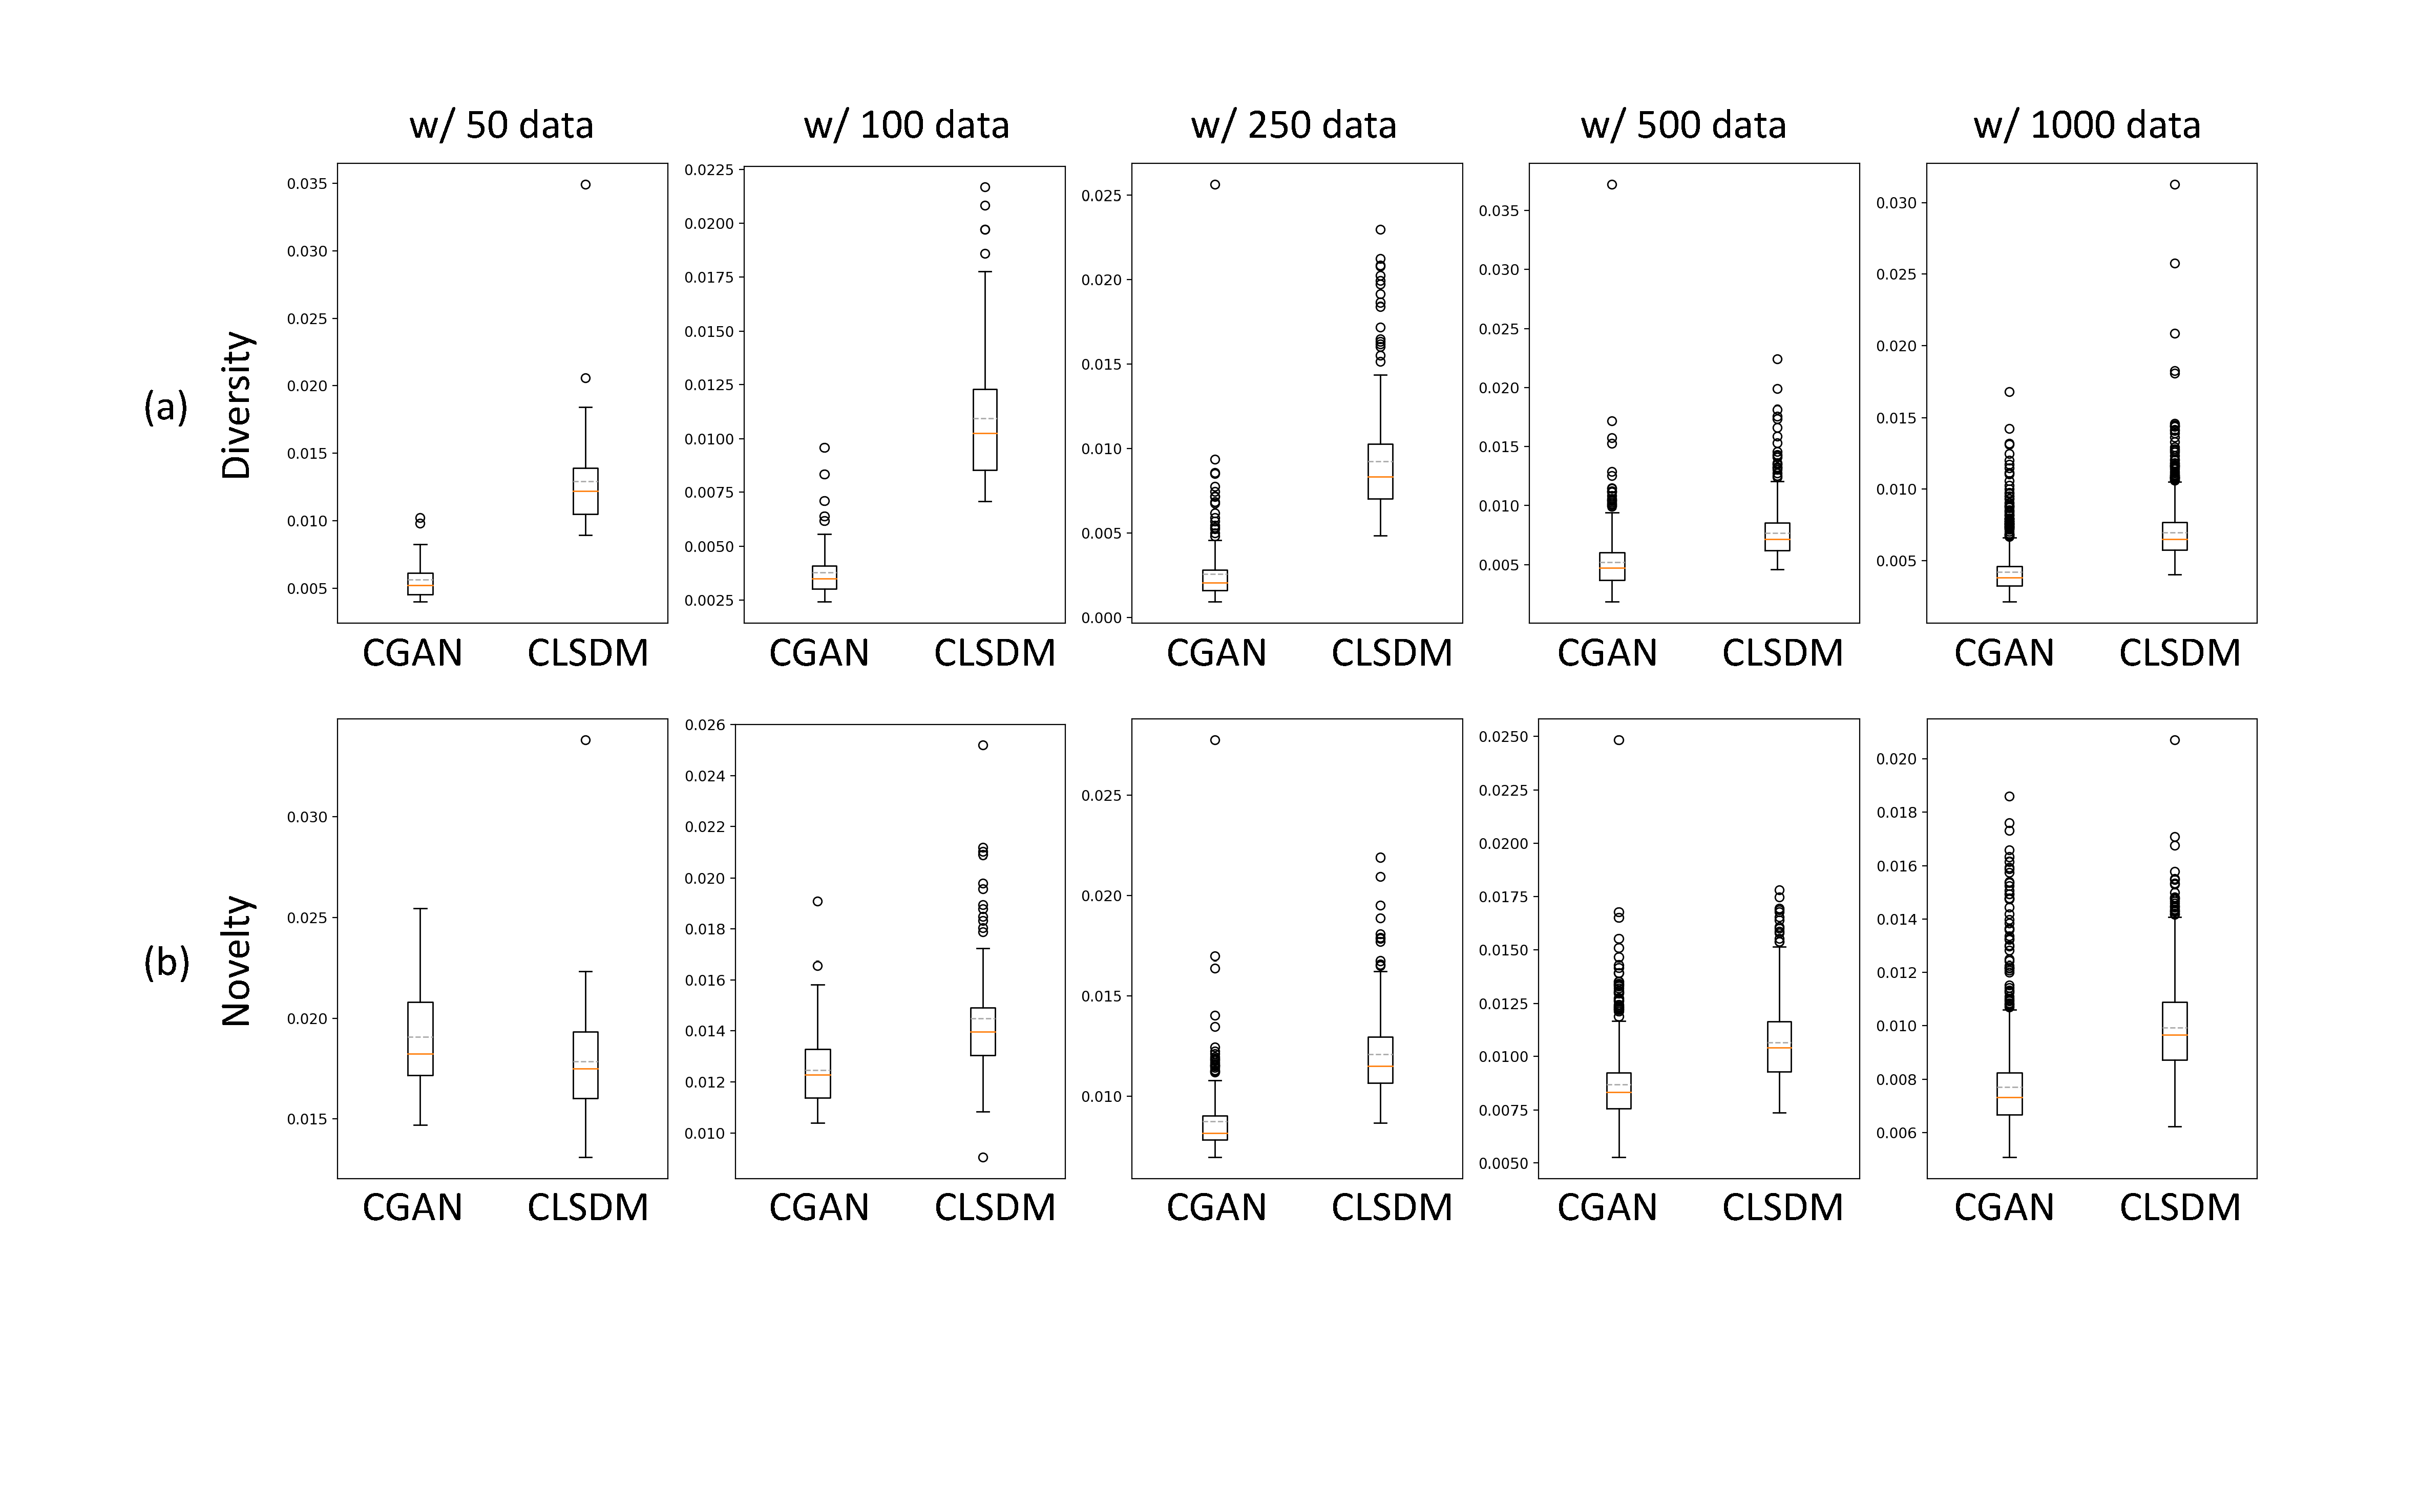
\includegraphics[width=0.95\linewidth]{chapter6/fig/conditional_inter_intra_dist.pdf}
    \end{center}
    \vspace{-2mm}
    \caption{
        \small Diversity ((a) $D_{intra}^{10}$) and novelty  ((b) $D_{inter}^{10}$) metrics for CGAN and CLSDM across dataset sizes.  
    }
    \label{ch6:fig:main_benchmark_conditional_intra_inter_dist}
\end{figure}

We also assess sampling exploration under conditioning to investigate whether the presence of a condition degrades diversity and novelty. By using the same $D^{10}_{intra}$ and $D^{10}_{inter}$ metrics, Fig.~\ref{ch6:fig:main_benchmark_conditional_intra_inter_dist} compares CLSDM and CGAN in terms of diversity and novelty of the conditioned samples. CLSDM generally maintains higher diversity and novelty than CGAN, similar to the unconditional case. Both models improve when given larger training sets, but CLSDM still shows better performance. Interestingly, CGAN’s novelty is higher at the lowest data setting with 50 samples. However, this is not due to CGAN exploring meaningfully, but rather because many CGAN outputs violate the area condition and effectively behave like unconstrained samples. These off-target shapes can appear “novel”, but they are not valid designs that satisfy the condition. In contrast, CLSDM’s samples adhere to the condition, so their novelty reflects the model's exploration within the constrained space.

In overall, \textit{DiffGeo}’s conditional diffusion CLSDM achieves a better balance between adherence to the condition and diversity of outputs. It supports the desired property with minimal sacrifice in variety, while the CGAN often either fails the condition or collapses the sampling diversity.

\subsubsection{Conclusion of Benchmarking}

The 2D benchmarking study addresses the research questions posed at the start of this section.

\begin{itemize}
    \item[1.] \textbf{Data Efficiency:} \textit{DiffGeo}, including LSDM and CLSDM, enables high-quality and diverse shape generation even with extremely limited training data. Unlike GANs, which require hundreds of samples to avoid model collapse, \textit{DiffGeo} produces realistic airfoils with as few as 50 training shapes, a nearly tenfold reduction in data requirements.

    \item[2.] \textbf{Deployment Flexibility:} The separation of geometric generative sampling and energy-based conditioning enables \textit{DiffGeo} to be reused without retraining. In the benchmark studies, introducing a new condition to switch from unconditional to conditional generation has no additional training cost, whereas GAN-based models had to be retrained.

    \item[3.] \textbf{Constraint Handling:} We showed that CLSDM can enforce an area constraint far more precise than a CGAN trained for the same purpose, and can be done with limited training data. 
\end{itemize}

In summary, \textit{DiffGeo} outperforms conventional GAN/VAE approaches as a data-driven shape sampler and provides a more data-efficient, flexible and controllable solution for design space exploration.